% Lines starting with a percent sign (%) are comments. LaTeX will 
% not process those lines. Similarly, everything after a percent 
% sign in a line is considered a comment. To produce a percent sign
% in the output, write \% (backslash followed by the percent sign). 
% ==================================================================
% Usage instructions:
% ------------------------------------------------------------------
% The file is heavily commented so that you know what the various
% commands do. Feel free to remove any comments you don't need from
% your own copy. When redistributing the example thesis file, please
% retain all the comments for the benefit of other thesis writers! 
% ==================================================================
% Compilation instructions: 
% ------------------------------------------------------------------
% Use pdflatex to compile! Input images are expected as PDF files.
% Example compilation:
% ------------------------------------------------------------------
% > pdflatex thesis-example.tex
% > bibtex thesis-example
% > pdflatex thesis-example.tex
% > pdflatex thesis-example.tex
% ------------------------------------------------------------------
% You need to run pdflatex multiple times so that all the cross-references
% are fixed. pdflatex will tell you if you need to re-run it (a warning
% will be issued)  
% ------------------------------------------------------------------
% Compilation has been tested to work in ukk.cs.hut.fi and kosh.hut.fi
% - if you have problems of missing .sty -files, then the local LaTeX
% environment does not have all the required packages installed.
% For example, when compiling in vipunen.hut.fi, you get an error that
% tikz.sty is missing - in this case you must either compile somewhere
% else, or you cannot use TikZ graphics in your thesis and must therefore
% remove or comment out the tikz package and all the tikz definitions. 
% ------------------------------------------------------------------

% General information
% ==================================================================
% Package documentation:
% 
% The comments often refer to package documentation. (Almost) all LaTeX
% packages have documentation accompanying them, so you can read the
% package documentation for further information. When a package 'xxx' is
% installed to your local LaTeX environment (the document compiles
% when you have \usepackage{xxx} and LaTeX does not complain), you can 
% find the documentation somewhere in the local LaTeX texmf directory
% hierarchy. In ukk.cs.hut.fi, this is /usr/texlive/2008/texmf-dist,
% and the documentation for the titlesec package (for example) can be 
% found at /usr/texlive/2008/texmf-dist/doc/latex/titlesec/titlesec.pdf.
% Most often the documentation is located as a PDF file in 
% /usr/texlive/2008/texmf-dist/doc/latex/xxx, where xxx is the package name; 
% however, documentation for TikZ is in
% /usr/texlive/2008/texmf-dist/doc/latex/generic/pgf/pgfmanual.pdf
% (this is because TikZ is a front-end for PGF, which is meant to be a 
% generic portable graphics format for LaTeX).
% You can try to look for the package manual using the ``find'' shell
% command in Linux machines; the find databases are up-to-date at least
% in ukk.cs.hut.fi. Just type ``find xxx'', where xxx is the package
% name, and you should find a documentation file.
% Note that in some packages, the documentation is in the DVI file
% format. In this case, you can copy the DVI file to your home directory,
% and convert it to PDF with the dvipdfm command (or you can read the
% DVI file directly with a DVI viewer).
% 
% If you can't find the documentation for a package, just try Googling
% for ``latex packagename''; most often you can get a direct link to the
% package manual in PDF format.
% ------------------------------------------------------------------


% Document class for the thesis is report
% ------------------------------------------------------------------
% You can change this but do so at your own risk - it may break other things.
% Note that the option pdftext is used for pdflatex; there is no
% pdflatex option. 
% ------------------------------------------------------------------
\documentclass[12pt,a4paper,oneside,pdftex]{report}

% The input files (tex files) are encoded with the latin-1 encoding 
% (ISO-8859-1 works). Change the latin1-option if you use UTF8 
% (at some point LaTeX did not work with UTF8, but I'm not sure
% what the current situation is) 
\usepackage[latin1]{inputenc}
% OT1 font encoding seems to work better than T1. Check the rendered
% PDF file to see if the fonts are encoded properly as vectors (instead
% of rendered bitmaps). You can do this by zooming very close to any letter 
% - if the letter is shown pixelated, you should change this setting 
% (try commenting out the entire line, for example).  
\usepackage[OT1]{fontenc}
% The babel package provides hyphenating instructions for LaTeX. Give
% the languages you wish to use in your thesis as options to the babel
% package (as shown below). You can remove any language you are not
% going to use.
% Examples of valid language codes: english (or USenglish), british, 
% finnish, swedish; and so on.
\usepackage[finnish,english]{babel}


% Font selection
% ------------------------------------------------------------------
% The default LaTeX font is a very good font for rendering your 
% thesis. It is a very professional font, which will always be 
% accepted. 
% If you, however, wish to spicen up your thesis, you can try out
% these font variants by uncommenting one of the following lines
% (or by finding another font package). The fonts shown here are 
% all fonts that you could use in your thesis (not too silly). 
% Changing the font causes the layouts to shift a bit; you many
% need to manually adjust some layouts. Check the warning messages
% LaTeX gives you.
% ------------------------------------------------------------------
% To find another font, check out the font catalogue from
% http://www.tug.dk/FontCatalogue/mathfonts.html
% This link points to the list of fonts that support maths, but
% that's a fairly important point for master's theses.
% ------------------------------------------------------------------
% <rant>
% Remember, there is no excuse to use Comic Sans, ever, in any
% situation! (Well, maybe in speech bubbles in comics, but there 
% are better options for those too)
% </rant>

% \usepackage{palatino}
% \usepackage{tgpagella}



% Optional packages
% ------------------------------------------------------------------
% Select those packages that you need for your thesis. You may delete
% or comment the rest.

% Natbib allows you to select the format of the bibliography references.
% The first example uses numbered citations: 
%\usepackage[square,sort&compress,numbers]{natbib}
% The second example uses author-year citations.
% If you use author-year citations, change the bibliography style (below); 
% acm style does not work with author-year citations.
% Also, you should use \citet (cite in text) when you wish to refer
% to the author directly (\citet{blaablaa} said blaa blaa), and 
% \citep when you wish to refer similarly than with numbered citations
% (It has been said that blaa blaa~\citep{blaablaa}).
%\usepackage[authoryear]{natbib}

\usepackage{bibentry}

\usepackage[round]{natbib}

\usepackage{multibib}
\newcites{src}{References}
%\newcites{pri}{Primary studies}

%\bibliographystyle{plainnat}
\bibliographystylesrc{plainnat}
\bibliographystyle{plainnat}


\usepackage{supertabular,array}  % useampisivuinen taulukko

%\bibliographystylepri{plainnat}
% The alltt package provides an all-teletype environment that acts
% like verbatim but you can use LaTeX commands in it. Uncomment if 
% you want to use this environment. 
% \usepackage{alltt}

% The eurosym package provides a euro symbol. Use with \euro{}
\usepackage{eurosym} 

% Verbatim provides a standard teletype environment that renderes
% the text exactly as written in the tex file. Useful for code
% snippets (although you can also use the listings package to get
% automatic code formatting). 
\usepackage{verbatim}

% The listing package provides automatic code formatting utilities
% so that you can copy-paste code examples and have them rendered
% nicely. See the package documentation for details.
% \usepackage{listings}

% The fancuvrb package provides fancier verbatim environments 
% (you can, for example, put borders around the verbatim text area
% and so on). See package for details.
% \usepackage{fancyvrb}

% Supertabular provides a tabular environment that can span multiple 
% pages. 
%\usepackage{supertabular}
% Longtable provides a tabular environment that can span multiple 
% pages. This is used in the example acronyms file. 
\usepackage{longtable}

% The fancyhdr package allows you to set your the page headers 
% manually, and allows you to add separator lines and so on. 
% Check the package documentation. 
% \usepackage{fancyhdr}

% Subfigure package allows you to use subfigures (i.e. many subfigures
% within one figure environment). These can have different labels and
% they are numbered automatically. Check the package documentation. 
\usepackage{subfigure}

% The titlesec package can be used to alter the look of the titles 
% of sections, chapters, and so on. This example uses the ``medium'' 
% package option which sets the titles to a medium size, making them
% a bit smaller than what is the default. You can fine-tune the 
% title fonts and sizes by using the package options. See the package
% documentation.
\usepackage[medium]{titlesec}

% The TikZ package allows you to create professional technical figures.
% The learning curve is quite steep, but it is definitely worth it if 
% you wish to have really good-looking technical figures. 
\usepackage{tikz}
% You also need to specify which TikZ libraries you use
\usetikzlibrary{positioning}
\usetikzlibrary{calc}
\usetikzlibrary{arrows}
\usetikzlibrary{decorations.pathmorphing,decorations.markings}
\usetikzlibrary{shapes}
\usetikzlibrary{patterns}


% The aalto-thesis package provides typesetting instructions for the
% standard master's thesis parts (abstracts, front page, and so on)
% Load this package second-to-last, just before the hyperref package.
% Options that you can use: 
%   mydraft - renders the thesis in draft mode. 
%             Do not use for the final version. 
%   doublenumbering - [optional] number the first pages of the thesis
%                     with roman numerals (i, ii, iii, ...); and start
%                     arabic numbering (1, 2, 3, ...) only on the 
%                     first page of the first chapter
%   twoinstructors  - changes the title of instructors to plural form
%   twosupervisors  - changes the title of supervisors to plural form
\usepackage[mydraft,twoinstructors]{aalto-thesis}
%\usepackage[mydraft,doublenumbering]{aalto-thesis}
%\usepackage{aalto-thesis}


% Hyperref
% ------------------------------------------------------------------
% Hyperref creates links from URLs, for references, and creates a
% TOC in the PDF file.
% This package must be the last one you include, because it has
% compatibility issues with many other packages and it fixes
% those issues when it is loaded.   
\RequirePackage[pdftex]{hyperref}
% Setup hyperref so that links are clickable but do not look 
% different
\hypersetup{colorlinks=false,raiselinks=false,breaklinks=true}
\hypersetup{pdfborder={0 0 0}}
\hypersetup{bookmarksnumbered=true}
% The following line suggests the PDF reader that it should show the 
% first level of bookmarks opened in the hierarchical bookmark view. 
\hypersetup{bookmarksopen=true,bookmarksopenlevel=1}
% Hyperref can also set up the PDF metadata fields. These are
% set a bit later on, after the thesis setup.   


%Custom packages added by me
%\usepackage{nameref} #Onnistuisko jos k�ytt�is vaan cleverrefi�
\usepackage{cleveref}
\usepackage{booktabs}
\usepackage{comment} 
%\usepackage{url}       % \url{...}

%\usepackage[usenames]{color} %t�� on kai ladattu jo jossain

%\newcommand{\basicalert}[2]{\fbox{\bfseries\sffamily\scriptsize\color{blue}
% #1}{\sf\small$\blacktriangleright$\textit{\color{red} #2}$\blacktriangleleft$} }
%\newcommand{\mika}[1]{\basicalert{From Mika}{#1}}
%\newcommand{\eetu}[1]{\basicalert{From Eetu}{#1}}
%\newcommand{\juha}[1]{\basicalert{From Juha}{#1}}
\newcommand{\mika}[1]{\ignorespaces}
\newcommand{\eetu}[1]{\ignorespaces}
\newcommand{\juha}[1]{\ignorespaces}



% Thesis setup
% ==================================================================
% Change these to fit your own thesis.
% \COMMAND always refers to the English version;
% \FCOMMAND refers to the Finnish version; and
% \SCOMMAND refers to the Swedish version.
% You may comment/remove those language variants that you do not use
% (but then you must not include the abstracts for that language)
% ------------------------------------------------------------------
% If you do not find the command for a text that is shown in the cover page or
% in the abstract texts, check the aalto-thesis.sty file and locate the text
% from there. 
% All the texts are configured in language-specific blocks (lots of commands
% that look like this: \renewcommand{\ATCITY}{Espoo}.
% You can just fix the texts there. Just remember to check all the language
% variants you use (they are all there in the same place). 
% ------------------------------------------------------------------
\newcommand{\TITLE}{Agile metrics:}
\newcommand{\FTITLE}{Ketter�t mittarit:}
%\newcommand{\STITLE}{Den stora stygga vargen:}
\newcommand{\SUBTITLE}{Why and how}
\newcommand{\FSUBTITLE}{Miksi ja miten}
%\newcommand{\SSUBTITLE}{Lilla Vargens universum}
\newcommand{\DATE}{June 18, 2011}
\newcommand{\FDATE}{18. kes�kuuta 2011}
%\newcommand{\SDATE}{Den 18 Juni 2011}

% Supervisors and instructors
% ------------------------------------------------------------------
% If you have two supervisors, write both names here, separate them with a 
% double-backslash (see below for an example)
% Also remember to add the package option ``twosupervisors'' or
% ``twoinstructors'' to the aalto-thesis package so that the titles are in
% plural.
% Example of one supervisor:
\newcommand{\SUPERVISOR}{Prof. Casper Lassenius}
\newcommand{\FSUPERVISOR}{Prof. Casper Lassenius}
%\newcommand{\SSUPERVISOR}{Professor Antti Yl�-J��ski}
% Example of twosupervisors:
%\newcommand{\SUPERVISOR}{Professor Antti Yl�-J��ski\\
  %Professor Pekka Perustieteilij�}
%\newcommand{\FSUPERVISOR}{Professori Antti Yl�-J��ski\\
  %Professori Pekka Perustieteilij�}
%\newcommand{\SSUPERVISOR}{Professor Antti Yl�-J��ski\\
  %Professor Pekka Perustieteilij�}

% If you have only one instructor, just write one name here
%\newcommand{\INSTRUCTOR}{Olli Ohjaaja M.Sc. (Tech.)}
%\newcommand{\FINSTRUCTOR}{Diplomi-insin��ri Olli Ohjaaja}
%\newcommand{\SINSTRUCTOR}{Diplomingenj�r Olli Ohjaaja}
% If you have two instructors, separate them with \\ to create linefeeds
\newcommand{\INSTRUCTOR}{Juha Itkonen D.Sc. (Tech.)\\
Mika M�ntyl� D.Sc. (Tech.)}
\newcommand{\FINSTRUCTOR}{Tkt Juha Itkonen\\
Tkt Mika M�ntyl�}
% \newcommand{\INSTRUCTOR}{Olli Ohjaaja M.Sc. (Tech.)\\
%  Elli Opas M.Sc. (Tech)}
%\newcommand{\FINSTRUCTOR}{Diplomi-insin��ri Olli Ohjaaja\\
%  Diplomi-insin��ri Elli Opas}
%\newcommand{\SINSTRUCTOR}{Diplomingenj�r Olli Ohjaaja\\
%  Diplomingenj�r Elli Opas}

% If you have two supervisors, it is common to write the schools
% of the supervisors in the cover page. If the following command is defined,
% then the supervisor names shown here are printed in the cover page. Otherwise,
% the supervisor names defined above are used.
%\newcommand{\COVERSUPERVISOR}{Professor Antti Yl�-J��ski, Aalto University\\
 % Professor Pekka Perustieteilij�, University of Helsinki}

% The same option is for the instructors, if you have multiple instructors.
% \newcommand{\COVERINSTRUCTOR}{Olli Ohjaaja M.Sc. (Tech.), Aalto University\\
%  Elli Opas M.Sc. (Tech), Aalto SCI}


% Other stuff
% ------------------------------------------------------------------
\newcommand{\PROFESSORSHIP}{Software Engineering}
\newcommand{\FPROFESSORSHIP}{Ohjelmistotuotanto ja -liiketoiminta}
%\newcommand{\SPROFESSORSHIP}{Datakommunikationsprogram}
% Professorship code is the same in all languages
\newcommand{\PROFCODE}{T3003}
\newcommand{\KEYWORDS}{agile, metrics}
\newcommand{\FKEYWORDS}{ketter�, mittarit}
%\newcommand{\SKEYWORDS}{oms�ttning, kassafl�de, v�rdepappersmarknadslagen,
%yrkesut�vare, intressef�retag, verifieringskedja}
\newcommand{\LANGUAGE}{English}
\newcommand{\FLANGUAGE}{Englanti}
%\newcommand{\SLANGUAGE}{Engelska}

% Author is the same for all languages
\newcommand{\AUTHOR}{Eetu Kupiainen}


% Currently the English versions are used for the PDF file metadata
% Set the PDF title
\hypersetup{pdftitle={\TITLE\ \SUBTITLE}}
% Set the PDF author
\hypersetup{pdfauthor={\AUTHOR}}
% Set the PDF keywords
\hypersetup{pdfkeywords={\KEYWORDS}}
% Set the PDF subject
\hypersetup{pdfsubject={Master's Thesis}}


% Layout settings
% ------------------------------------------------------------------

% When you write in English, you should use the standard LaTeX 
% paragraph formatting: paragraphs are indented, and there is no 
% space between paragraphs.
% When writing in Finnish, we often use no indentation in the
% beginning of the paragraph, and there is some space between the 
% paragraphs. 

% If you write your thesis Finnish, uncomment these lines; if 
% you write in English, leave these lines commented! 
% \setlength{\parindent}{0pt}
% \setlength{\parskip}{1ex}

% Use this to control how much space there is between each line of text.
% 1 is normal (no extra space), 1.3 is about one-half more space, and
% 1.6 is about double line spacing.  
% \linespread{1} % This is the default
% \linespread{1.3}

% Bibliography style
% acm style gives you a basic reference style. It works only with numbered
% references.
%\bibliographystyle{acm}
% Plainnat is a plain style that works with both numbered and name citations.
%\bibliographystyle{plainnat}



% Extra hyphenation settings
% ------------------------------------------------------------------
% You can list here all the files that are not hyphenated correctly.
% You can provide many \hyphenation commands and/or separate each word
% with a space inside a single command. Put hyphens in the places where
% a word can be hyphenated.
% Note that (by default) LaTeX will not hyphenate words that already
% have a hyphen in them (for example, if you write ``structure-modification 
% operation'', the word structure-modification will never be hyphenated).
% You need a special package to hyphenate those words.
\hyphenation{di-gi-taa-li-sta yksi-suun-tai-sta}



% The preamble ends here, and the document begins. 
% Place all formatting commands and such before this line.
% ------------------------------------------------------------------
\begin{document}
% This command adds a PDF bookmark to the cover page. You may leave
% it out if you don't like it...
\pdfbookmark[0]{Cover page}{bookmark.0.cover}
% This command is defined in aalto-thesis.sty. It controls the page 
% numbering based on whether the doublenumbering option is specified
\startcoverpage

% Cover page
% ------------------------------------------------------------------
% Options: finnish, english, and swedish
% These control in which language the cover-page information is shown
\coverpage{english}


\nobibliography{sources_p}

% Abstracts
% ------------------------------------------------------------------
% Include an abstract in the language that the thesis is written in,
% and if your native language is Finnish or Swedish, one in that language.

% Abstract in English
% ------------------------------------------------------------------
%\begin{comment}
\thesisabstract{english}{
A dissertation or thesis is a document submitted in support of candidature
for a degree or professional qualification presenting the author's research and
findings. In some countries/universities, the word thesis or a cognate is used
as part of a bachelor's or master's course, while dissertation is normally
applied to a doctorate, whilst, in others, the reverse is true.

%\citetsrc{1579312}
} 

%\end{comment}

% Abstract in Finnish
% ------------------------------------------------------------------
\thesisabstract{finnish}{
Kivi on materiaali, joka muodostuu mineraaleista ja luokitellaan
}

% Acknowledgements
% ------------------------------------------------------------------
% Select the language you use in your acknowledgements
\selectlanguage{english}

% Uncomment this line if you wish acknoledgements to appear in the 
% table of contents
%\addcontentsline{toc}{chapter}{Acknowledgements}

% The star means that the chapter isn't numbered and does not 
% show up in the TOC
\chapter*{Acknowledgements}

I wish to thank all students who use \LaTeX\ for formatting their theses,

\vskip 10mm

\noindent Espoo, \DATE
\vskip 5mm
\noindent\AUTHOR

% Acronyms
% ------------------------------------------------------------------
% Use \cleardoublepage so that IF two-sided printing is used 
% (which is not often for masters theses), then the pages will still
% start correctly on the right-hand side.
\cleardoublepage
% Example acronyms are placed in a separate file, acronyms.tex
\addcontentsline{toc}{chapter}{Abbreviations and Acronyms}
\chapter*{Abbreviations and Acronyms}

% The longtable environment should break the table properly to multiple pages, 
% if needed

\noindent
\begin{longtable}{@{}p{0.25\textwidth}p{0.7\textwidth}@{}}
SLR & Systematic literature review
WIP & Work in progress
\fixme{Poista koko abbreviations jos ei tuu montaa}


\end{longtable}


% Table of contents
% ------------------------------------------------------------------
\cleardoublepage
% This command adds a PDF bookmark that links to the contents.
% You can use \addcontentsline{} as well, but that also adds contents
% entry to the table of contents, which is kind of redundant.
% The text ``Contents'' is shown in the PDF bookmark. 
\pdfbookmark[0]{Contents}{bookmark.0.contents}
\tableofcontents

% List of tables
% ------------------------------------------------------------------
% You only need a list of tables for your thesis if you have very 
% many tables. If you do, uncomment the following two lines.
% \cleardoublepage
% \listoftables

% Table of figures
% ------------------------------------------------------------------
% You only need a list of figures for your thesis if you have very 
% many figures. If you do, uncomment the following two lines.
% \cleardoublepage
% \listoffigures

% The following label is used for counting the prelude pages
\label{pages-prelude}
\cleardoublepage

%%%%%%%%%%%%%%%%% The main content starts here %%%%%%%%%%%%%%%%%%%%%
% ------------------------------------------------------------------
% This command is defined in aalto-thesis.sty. It controls the page 
% numbering based on whether the doublenumbering option is specified
\startfirstchapter

% Add headings to pages (the chapter title is shown)
\pagestyle{headings}

% The contents of the thesis are separated to their own files.
% Edit the content in these files, rename them as necessary.
% ------------------------------------------------------------------
\chapter{Introduction}
\label{chapter:intro}
 % Software engineering is at a crossroads as there are new leaner and more
% agile software development methods appearing next to the traditional
% software development methods.
% \mika{Kappaleen pointti: No literature reviews of actual metric use}
Software metrics have been studied for decades and several literature reviews
have been published.
Yet, the literature reviews have been written from an academic viewpoint that
typically focuses on the effectiveness of a single metric. For example, Catal
et al. review fault prediction metrics \citepsrc{catal2009systematic},
\citetsrc{purao2003product} review metrics for object oriented systems and
\citetsrc{kitchenham_whats_2010} performs a mapping of most cited software
metrics papers. According to the researcher's knowledge there are no
systematic literature reviews on the actual use of software metrics in the
industry.

%\mika{Kappaleen pointti: Agile on t�rke�� eik� metriikkoja tutkittu}

% \juha{Yritin konkretisoida trad vs. agile kontrastia}
Agile software development is becoming increasingly popular in the software
industry. The agile approach seems to be contradicting with the traditional
metrics approaches. For example, the agile emphasizes working software over
measuring progress in terms of intermediate products or documentation, and
embracing the change invalidates the traditional approach of tracking progress
against pre-made plan.
However, at the same time agile software development highlights some measures
that should be used, e.g., burndown graphs and 100\% automated unit testing
coverage. However, measurement research in the context of agile methods
remains scarce.

The goal of this paper is to review the literature of actual use of software
metrics in the context of agile software development. This study will lay out
the current state of metrics usage in industrial agile software development
based on literature.
Moreover, the study uncovers the reasons for metric usage as well as
highlights actions that the use of metrics can trigger.
%Due to our research
%goal, we focus this paper on case studies and actual empirical findings
%excluding theoretical discussion and models lacking empirical validation.

This study covers the following research questions: 

\begin{itemize}
  \item RQ1: Why are metrics used?
  \item RQ2: What actions do the use of metrics trigger?
  \item RQ3: Which metrics are used?
  \item RQ4: What metrics are important?
\end{itemize} 

%\section{Problem statement}

\section{Structure of the Thesis}
\label{section:structure} 

This thesis is structured as follows. \Cref{sec:Method} describes how
the SR was conducted. \Cref{sec:Results} reports the results from the study.
\Cref{sec:Discussion} discusses about the findings and how they map to agile
principles. \Cref{sec:Conclusions} concludes the paper. \fixme{Final
structure}

\chapter{Background}

\section{Agile software development}
%\eetu{t�ss� voisi olla historian�k�kulma, voipi menn� pitk�ks eik� niin
%mielenkiintoinen ehk� t�ss� paperissa} 

Agile development methods have emerged to the software world ruled by
traditional heavyweight methods. In agile methods the focus is in lightweight
working practices, constant deliveries and customer collaboration over long
planning periods, heavy documentation and inflexible development phases.

Agile manifesto created by agile enthusiasts \citepsrc{beck2001agile} lists
agile principles that give an idea what is agile development about. Popular agile
development methods include Scrum \citepsrc{schwaber2002agile}, Extreme
Programming \citepsrc{beck2004extreme} and Kanban
\citepsrc{anderson2010kanban}.

%\section{Software measurement}
%Measurements for software industry started from a technical point of view.

\section{Related work}

\citetsrc{1667571} don't provide any specific agile metrics but rather
describes how agile metrics should be chosen and how they should be introduced
to the organization. Also, they provide a set of heuristics for agile metrics.


\fixme{t�� j�i v�h�n laihaks}

\section{Systematic literature review}

Systematic literature review is a research method originated from the field of
medicine \fixme{viite}. The overarching idea is to aggregate and synthetisize
existing knowledge regarding a research topic. This rigorous and audible
evaluation method can facilitate theory development and point out gaps in
research \citepsrc{webster2002analyzing}.

\section{Causes for software project failures}


\section{Evidence based software engineering}

%\subsection{Measurement}
%According to Fenton et al.\cite{fenton1998software} ``Measurement is the
%process by which numbers of symbols are assigned to attributes of entities in
%the real world in such way as to describe them according to clearly defined
%rules.''


\section{Previous metric research}

%There are a few mapping studies on software metrics(t�h�n vois lis�t� ne
% kitch whats 2010:ss� olevat muut mut en tii� mit� lis�arvoa ne tois).
%\cite{kitchenham_whats_2010} says there is a large body of research related
% to software metrics. However, she highlights that all evidence should be
%critically appraised so that further studies can be based on good quality
%evidence. She also reminds researchers to understand the context where
% metrics are taken from - failure to understand context will probably not provide
%answers to industry-related questions. 

%--EBSE
%--Mittaamisen SR:t
%--Agile mittaamisen muut tutkimukset vai enemm�nkin tutkimuksessa k�ytettyjen
%termien ja k�sitteiden selitt�minen


%\section{Aims and research questions} 
%The aim of this paper is to provide
% preliminary results from a systematic review (SR) on agile metrics.
%Moreover, we are interested on the industrial use of metrics in agile
% context.

\chapter{Review method}
\label{sec:Method}
Systematic review (SR) was chosen as research method because the study is more
about trying to understand a problem instead of trying to find a solution to
it. Also, there was already existing literature that could be synthesized.

\section{Protocol development}
Kitchenham's guide for SRs \citepsrc{kitchenham2004procedures} was used as a
basis for developing the review protocol. Additionally, a SR on agile
development \citepsrc{dyba_empirical_2008} and a SR on SR
\citepsrc{kitchenham2013systematic} were used to further understand the
challenges and opportunities of SRs. The protocol was also iterated in weekly
meetings with the instructors, as well as in a pilot study.

%otherguidelines \cite{webster2002analyzing}, a lessons learned from SRs
% \cite{brereton2007lessons},
\section{Search and selection process}

The strategy for finding primary studies was following:

\begin{itemize}
  \item Stage 1: Automated search
  \item Stage 2: Selection based on title and abstract
  \item Stage 3: Selection based on full text. Conduct data
  extraction and quality assessment.
\end{itemize}

\Cref{SelectionFunnel} shows the selection funnel in terms of the number
of papers after each stage.

%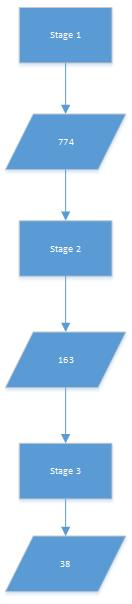
\includegraphics{SelectionFunnel.jpg}

\begin{table}
\centering
\caption{Paper selection funnel}
\begin{tabular}{|l|c|r} \hline
\label{SelectionFunnel}
Stage & Amount of papers \\ \hline
Stage 1 & 774 \\  
Stage 2 & 163 \\ 
Stage 3 & 29\\
\hline
\end{tabular}
\end{table}

% \subsubsection{Search strings}
Scopus database \footnote{http://www.scopus.com} was used to find the primary
documents with automated search. Keywords include popular agile development
methods and synonyms for the word metric. The search was improved
incrementally in three phases because some key papers and XP
conferences were not found initially. The search strings, hits and dates can
be found from \cref{app:Strings}.

%\juha{Laittaisin my�s inclusion ja exclusion kriteerit appendixiin ja
% j�tt�isin vain t�m�nkaltaisen lyhyen kuvauksen t�nne} 
The selection of the primary documents was based on inclusion criteria:
\emph{papers that present empirical findings on the industrial use and
experiences of metrics in agile context.} The papers were excluded based on
multiple criteria, mainly due to not conforming to requirements regarding
empirical findings and agile and industrial context. Full criteria are listed
in \cref{app:Criteria}.

%\juha{Inclusion criteria ja exclusion criteria siirretty -> appendix}
%\subsubsection{Inclusion criteria} \juha{->APPENDIX}
%
%\begin{itemize}
%  \item Papers that present the use and experiences of metrics in an agile
%  industry setting.
%\end{itemize}
%
%\subsubsection{Exclusion criteria} \juha{->APPENDIX}
%
%\begin{itemize}
%  \item Papers that don't contain empirical data from industry cases.
%  \item Papers that are not in English.
%  \item Papers that don't have agile context. There is evidence of
%  clearly non-agile practices or there is no agile method named. For example,
%  paper mentions agile but case company has only three releases per year.
%  \item Paper is only about one agile practice, which is not related to
%  measuring.
%  \item Papers that don't seem to have any data about metric usage. Similarly,
%  if there are only a few descriptions of metrics but no other info regarding
%  reasons or usage.
%  \item Papers that have serious issues with grammar or vocabulary and
%  therefore it takes considerable effort to understand sentences.
%  \item Papers that refer to another paper where the actual case is discussed.
%  \item Papers that are in academic or semi-academic setting - customer or
%  part of workers are from industry. The reason for this is that it doesn't
%  fully represent industry setting as software development methods are likely
%  enforced by academia.
%  \item Papers where results cannot be separated by setting, for example
%  surveys where there is data both from academia and industry. Similar
%  exclusion if results cannot be separated by software development method. 
%  \item Papers where the setting is not clear. For example only mention of
%  context is ``100 junior developers''.
%  \item Papers that are full conference proceedings. Individual papers should
%  be already listed separately.
%  \item Papers where the measurements are only used for the research. For
%  example author measures which agile practices correlate with success.
%  \item Papers that don't even show measurement usage in a pilot setting. For
%  example method or metric is used against static industrial data set.
%  %\item Papers that are about the same case, from the same author and same
%  %research focus, basically the paper format has just changed slightly.
%\end{itemize}


%\subsubsection{Stage 1 - Automatic search}

In stage 1, Scopus was used as the only search engine as it contained the most
relevant databases IEEE and ACM. Also, it was able to find Agile and XP conference
papers. Only XP Conference 2013 was searched manually because it couldn't be
found through Scopus.

%\subsubsection{Pilot}
%\label{pilot}
%We conducted a pilot study in order to refine the aim of the research and get
%familiar with the research method. Moreover, it was possible to modify the
%method and tools.

%15 papers were selected for the pilot; 5 by relevance, 5 by number of
%citations, and 5 by random selection.
% \begin{itemize} \item 5 by top relevance \item 5 by top citations \item 5 by
% random \end{itemize}
%\juha{t�m� mahdollista poistaa (ainakin omana alilukuna) jos tila ei
% riit�}The pilot resulted in changing citation manager tool from Zotero to Jabref.
%Also, selection by title and selection by abstract steps were joined
% together.
%The quality assessment checklist was decided based on the pilot results.

%\subsubsection{Stage 2 - Selection by title and abstract}

In stage 2, papers were included and excluded by the researcher based on their
title and abstract. As the quality of abstracts can be poor in computer
science \citepsrc{kitchenham2004procedures}, full texts were also skimmed
through in case of unclear abstracts.
% - especially introduction, case description and conclusions were checked
% briefly.
Unclear cases were discussed with the instructors in weekly meetings and an
exclusion rule was documented if necessary.

The validity of the selection process was analysed by performing the selection
for a random sample of 26 papers also by the second instructor. The level of
agreement was 'substantial' with Kappa 0.67
\citepsrc{landis_measurement_1977}.

%\subsubsection{Stage 3 - Selection by full text}

Stage 3 included multiple activities in one work flow. Selection by full text
was done, data was coded and quality assessment was done. Once again, if there
were unclear papers, they were discussed in meetings. Also, selection of 7
papers was conducted by the second instructor with an 'almost perfect'
agreement, Kappa 1.0 \citepsrc{landis_measurement_1977}.

\section{Data extraction}

Integrated coding was selected for data extraction strategy
\citepsrc{6092576}.
It provided focus to research questions but flexibility regarding findings.
Deductive coding would have been too restraining and inductive coding might
have caused too much bias. Integrated coding made it possible to create a
sample list of code categories:

\begin{itemize}
  \item Why is measurement used?
  \item How is measurement used?
  \item Metric
  \item Importance related to metric
  \item Context
\end{itemize}

The coding started with the researcher reading the full text and marking
interesting quotes with a temporary code. After, reading the full text the
researcher checked each quote and coded again with an appropriate code based
on the built understanding. In weekly meetings with the instructors, a rule
set for collecting metrics was slowly built:

\begin{itemize}
  \item Collect metric if team or company uses it.
  \item Collect metric only if something is said about why it is used, what
  actions it causes or if it is described as important.
  \item Don't collect metrics that are only used for the comparison and
  selection of development methods. 
  \item Don't collect metrics that are primarily used to compare teams. 
\end{itemize}

Atlas.ti Visual QDA (Qualitative Data Analysis), version 7.1.x was used to
collect and synthesize the qualitative data. Amount of found quotes per code
can be seen in \Cref{tab:quotes}.

To evaluate the repeatability of finding the same metrics, second instructor
coded metrics from three papers. Capture-recapture method
\citepsrc{seber2002estimation} was then used which showed that 90\% of metrics
were found.

% Table generated by Excel2LaTeX from sheet 'Taul1'
\begin{table}[htbp]
  \centering
  \label{tab:quotes}
  \caption{Amount of found quotes}
    \begin{tabular}{rr}
    \toprule
    Code  & Amount of quotations \\
    \midrule
    Why use this metric? & 151 \\
    How is measurement used? & 61 \\
    Metrics & 108 \\
    Importance related to metric & 45 \\
    Context & 158 \\
    \bottomrule
    \end{tabular}%
  \label{tab:addlabel}%
\end{table}%



A quality assessment form adopted from \citepsrc{dyba_empirical_2008} was used
to evaluate the quality of each primary study. Detailed list of quality
assessment questions can be found in \cref{app:quality}. Additionally, a
relevancy factor was added to the same assessment to describe how useful the
paper was for this study. The scale for the relevancy factor is:

\begin{itemize}
  \item 0 = doesn't contain any information regarding metrics and should be
  already excluded
  \item 1 = only descriptions of metrics with no additional info
  \item 2 = some useful information related to metrics
  \item 3 = a good amount of relevant information regarding metrics and metric
  usage
\end{itemize}

\section{Data synthesis}
Data synthesis followed the steps recommended by \citetsrc{6092576}.
Process started by going through all quotes within one code and giving each quote a
more descriptive code describing the quote in high level. Then the descriptive
codes were organized in groups based on their similarity. These groups were
then given high level codes which are seen as categories in
\cref{WhyHowCategories}.


\chapter{Results} % - Why and how are metrics used
\label{sec:Results}

This chapter presents the results from the systematic literature 
review. \Cref{PublicationDistribution} shows the distribution of primary
studies by publication channels. \Cref{tab:AgileMethods} lists the
distribution of agile methods and \Cref{tab:Domains} lists the distribution of
domains. %Distribution of metrics are listed in \cref{app:Metrics}.

\section{Overview of studies}

\begin{table}
\centering
\caption{Publication distribution of primary studies}
\label{PublicationDistribution}
\begin{tabular}{llll}
\hline Publication channel & Type & \# & \%\\
\hline Agile Conference & Conference & 8 & 38\\
HICCS & Conference & 3 & 14\\
ICSE & Workshop & 2 & 10\\
XP Conference & Conference & 2 & 10\\
Agile Development Conference & Conference & 1 & 5\\
APSEC & Conference & 1 & 5\\
ASWEC & Conference & 1 & 5\\
%ECIS & Conference & 1 & 5\\
%ECSA & Conference & 1 & 5\\ 
Elektronika ir Elektrotechnika & Journal & 1 & 5\\
Empirical Software Engineering & Journal & 1 & 5\\
EUROMICRO & Conference & 1 & 5\\
ICSE & Conference & 1 & 5\\
ICSP & Conference & 1 & 5\\
%ICSSP & Conference & 1 & 5\\
IST & Journal & 1 & 5\\
IJPQM & Journal & 1 & 5\\
JSS & Journal & 1 & 5\\
PROFES & Conference & 1 & 5\\
Software - Prac. and Exp. & Journal & 1 & 5\\
WETSoM & Workshop & 1 & 5\\
\hline

\end{tabular}
\end{table}


% Table generated by Excel2LaTeX from sheet 'Taul1'
\begin{table}[htbp]
  \centering
  \caption{Distribution of research methods}
    \begin{tabular}{rr}
    \toprule
    Research method & Amount \\
    \midrule
    Multicase & 2 \\
    Experience report & 7 \\
    Singlecase & 19 \\
    Survey & 1 \\
    \bottomrule
    \end{tabular}%
  \label{tab:ResearchMethods}%
\end{table}%


% Table generated by Excel2LaTeX from sheet 'Taul1'
\begin{table}[htbp]
  \centering
  \caption{Distribution of agile methods}
    \begin{tabular}{rr}
    \toprule
    Agile method & Amount \\
    \midrule
    Scrum & 15 \\
    XP    & 7 \\
    Lean  & 5 \\
    Other & 5 \\
    \bottomrule
    \end{tabular}%
  \label{tab:AgileMethods}%
\end{table}%

% Table generated by Excel2LaTeX from sheet 'Taul1'
\begin{table}[htbp]
  \centering
  \caption{Distribution of domains}
    \begin{tabular}{rr}
    \toprule
    Domain & Amount \\
    \midrule
    Telecom & 10 \\
    Enterprise information system & 7 \\
    Web application & 4 \\
    Other & 11 \\
    \bottomrule
    \end{tabular}%
  \label{tab:Domains}%
\end{table}%



\begin{comment}
\begin{table*}
%\centering
\caption{Overview of primary studies}
\label{OverviewOfPdocs} 
\begin{tabular}{lllllp{3cm}p{8cm}} \hline
ID & Year & Resear. meth. & Agile method & Team size & Domain & Metrics\\
\hline 
\cite{S3} & 2009 & Multicase &  NA/Scrum/Scrum & 2-10/2-7/4-8
& ERP/Graphic design plug-in/Facility management & Team available hours, team
effective hours, critical defects sent by customer, open defects, test
failure rate\\
\cite{S4} & 2013 & Experience r. & Scrum & 25 teams & Software
for oil and gas industry & Technical debt in categories, build status,
technical debt in effort\\
\cite{S5} & 2005 & Singlecase & XP & 15 & Enterprise information
system & Burndown, check-ins per day, number of automated test steps, faults
per iteration\\
[S6] & 2002 & Experience r. & XP & 50 & Enterprise
resource solution for the leasing industry & Velocity\\
\cite{S7} & 2011 & Survey & Scrum & 26 teams & Desktop and SaaS
products & Burndown, story points, \# of open defects, defects found in
system test, defects deferred, net promoter score\\
\cite{S8} & 2010 & Experience r. & Scrum & 5-9 & NA & Story
points, task effort, velocity\\
\cite{S9} & 2006 & Singlecase & XPMix & 15-20 & Broadband order
system & Effort estimate, actual effort\\
\cite{S10} & 2004 & Multicase & XP/Scrum & 4-18/6-9 &
b-2-b e-commerce solutions/Criminal justice system development & \# of
defects/velocity\\
\cite{S11} & 2007 & Singlecase & ScrumMix & 500 & Security
services & Revenue per customer\\
\cite{S12} & 2010 & Singlecase & ScrumMix & NA & E-commerce & Task
expected start and end date, effort estimate, completed web pages, task done\\
\cite{S13} & 2011 & Singlecase &
LeanScrumFDD & 5$\pm$2 & Information and communication software development & Fix time of failed
build, story flow percentage, percentage of stories prepared for sprint,
time to establish project foundation, velocity of elaborating features,
velocity of implementing features\\
\cite{S14} & 2012 & Experience r. & XPMix & NA & Web application
development & Broken build, test coverage, test growth ratio, violations of
static code checks, \# of unit tests\\
\cite{S16} & 2012 & Singlecase & Scrum & 6-8 &Web page development
& Sprint velocity, release velocity, cost performance index, schedule
performance index, planned velocity\\
\cite{S17} & 2007 & Singlecase & Lean & Comp. 160 devs& Various
& Common tempo time, number of bounce backs, cycle time, work in progress\\
\cite{S18} & 2010 & Singlecase & ScrumXPMix & Dev site 600 &
Telecom & Lead time, processing time, queue time\\
\cite{S19} & 2010 & Singlecase & AgileMix & 6-7 & Telecom &
Change request per requirement, fault slips, implemented vs wasted
requirements, maintenance effort\\
\cite{S21} & 2011 & Singlecase & ScrumXPMix & Dev site 500 &
Telecom & Rate of requirements per phase, variance in handovers,
requirement's cost types\\
\cite{S22} & 2012 & Singlecase & LeanMix & NA & Telecom &
Cumulative flow of maintenance requests, lead time\\
\cite{S20} & 2010 &  Singlecase & LeanMix & NA & Telecom &
\# of faults, fault-slip-through, \# of requests from customer,
\# of requirements per phase\\
[S23] & 2011 & Experience r. & AgileMix & 9 and 6 & 
Casino games & Work in progress, average velocity, cycle time\\
\cite{S24} & 2011 & Singlecase & ScrumBan & 6-8 & Telecom
maintenance & Lead time, work in progress, \# of days in maintenance,
\# of days to overdue, reported hours on CSR\\
%\cite{Shen200725} & 2007 & Singlecase & ScrumXPMix & 4 & Independent software
% developer & Adaptability, innovation, productivity, ROI\\
\cite{S26} & 2011 & Singlecase & LeanMix & project size 200 & Telecom
& Throughput\\
\cite{S25} & 2010 & Singlecase & LeanMix & project size 100 &
Telecom & Defect trend indicator, \# of defects, predicted \# of
defects\\
\cite{S28} & 2009 & Singlecase & XP & 15 & Enterprise information
system & Burndown, check-ins per day, number of automated test steps\\
\cite{S27} & 2006 & Singlecase & XPMix & 15 & Enterprise information
system & Burndown, \# of new defects, number of written and passed tests,
task estimated vs actual time, time reported for overhead activities,
check-ins per day\\
\cite{S29} & 2006 &  Experience r. & ScrumXPMix & NA & Telecom
& Story estimate, story complete percentage\\
\cite{S30} & 2013 & Singlecase & ScrumMix & 5 & Space mission
control software & Progress as working code\\
\cite{S31} & 2006 & Experience r. & DSDM & NA & Library software &
Costs, schedule\\
\hline
\end{tabular}
\end{table*}
\end{comment}

\subsection{Quality of studies}

% Table generated by Excel2LaTeX from sheet 'Taul1'
\begin{table}[htbp]
  \centering
  \caption{Quality assessment fo primary studies}
    \begin{tabular}{rp{0,5cm}p{0,5cm}p{0,5cm}p{0,5cm}p{0,5cm}p{0,5cm}p{0,5cm}p{0,5cm}p{0,5cm}p{0,5cm}p{0,5cm}p{0,5cm}p{0,5cm}}
    \toprule
    Study & Rese arch & Aim   & Con text & R.de sign & Samp ling & Ctrl. Grp & Data coll. & Data anal & Reflex ivity & Find ings & Value & Total & Rele vancy \\
    \midrule
     {[}S1{]} & \multicolumn{1}{l}{1} & \multicolumn{1}{l}{1} & \multicolumn{1}{l}{1} & \multicolumn{1}{l}{1} & \multicolumn{1}{l}{1} & \multicolumn{1}{l}{0} & \multicolumn{1}{l}{1} & \multicolumn{1}{l}{1} & \multicolumn{1}{l}{1} & \multicolumn{1}{l}{1} & \multicolumn{1}{l}{1} & 10    & \multicolumn{1}{l}{2} \\
     {[}S2{]} & \multicolumn{1}{l}{0} & \multicolumn{1}{l}{0} & \multicolumn{1}{l}{0} & \multicolumn{1}{l}{0} & \multicolumn{1}{l}{1} & \multicolumn{1}{l}{0} & \multicolumn{1}{l}{0} & \multicolumn{1}{l}{0} & \multicolumn{1}{l}{0} & \multicolumn{1}{l}{0} & \multicolumn{1}{l}{1} & 2     & \multicolumn{1}{l}{2} \\
     {[}S3{]} & \multicolumn{1}{l}{1} & \multicolumn{1}{l}{1} & \multicolumn{1}{l}{0} & \multicolumn{1}{l}{1} & \multicolumn{1}{l}{0} & \multicolumn{1}{l}{0} & \multicolumn{1}{l}{0} & \multicolumn{1}{l}{0} & \multicolumn{1}{l}{0} & \multicolumn{1}{l}{0} & \multicolumn{1}{l}{0} & 3     & \multicolumn{1}{l}{2} \\
     {[}S4{]} & \multicolumn{1}{l}{0} & \multicolumn{1}{l}{0} & \multicolumn{1}{l}{0} & \multicolumn{1}{l}{0} & \multicolumn{1}{l}{1} & \multicolumn{1}{l}{0} & \multicolumn{1}{l}{0} & \multicolumn{1}{l}{0} & \multicolumn{1}{l}{0} & \multicolumn{1}{l}{0} & \multicolumn{1}{l}{1} & 2     & \multicolumn{1}{l}{3} \\
     {[}S5{]} & \multicolumn{1}{l}{1} & \multicolumn{1}{l}{1} & \multicolumn{1}{l}{1} & \multicolumn{1}{l}{1} & \multicolumn{1}{l}{1} & \multicolumn{1}{l}{0} & \multicolumn{1}{l}{1} & \multicolumn{1}{l}{1} & \multicolumn{1}{l}{0} & \multicolumn{1}{l}{1} & \multicolumn{1}{l}{1} & 9     & \multicolumn{1}{l}{3} \\
     {[}S6{]} & \multicolumn{1}{l}{0} & \multicolumn{1}{l}{0} & \multicolumn{1}{l}{1} & \multicolumn{1}{l}{0} & \multicolumn{1}{l}{1} & \multicolumn{1}{l}{0} & \multicolumn{1}{l}{0} & \multicolumn{1}{l}{0} & \multicolumn{1}{l}{0} & \multicolumn{1}{l}{0} & \multicolumn{1}{l}{1} & 3     & \multicolumn{1}{l}{2} \\
     {[}S7{]} & \multicolumn{1}{l}{0} & \multicolumn{1}{l}{0} & \multicolumn{1}{l}{0} & \multicolumn{1}{l}{0} & \multicolumn{1}{l}{0} & \multicolumn{1}{l}{1} & \multicolumn{1}{l}{1} & \multicolumn{1}{l}{1} & \multicolumn{1}{l}{0} & \multicolumn{1}{l}{1} & \multicolumn{1}{l}{1} & 5     & \multicolumn{1}{l}{2} \\
     {[}S8{]} & \multicolumn{1}{l}{0} & \multicolumn{1}{l}{0} & \multicolumn{1}{l}{0} & \multicolumn{1}{l}{0} & \multicolumn{1}{l}{0} & \multicolumn{1}{l}{1} & \multicolumn{1}{l}{0} & \multicolumn{1}{l}{0} & \multicolumn{1}{l}{0} & \multicolumn{1}{l}{1} & \multicolumn{1}{l}{1} & 3     & \multicolumn{1}{l}{3} \\
     {[}S9{]} & \multicolumn{1}{l}{1} & \multicolumn{1}{l}{1} & \multicolumn{1}{l}{1} & \multicolumn{1}{l}{1} & \multicolumn{1}{l}{0} & \multicolumn{1}{l}{0} & \multicolumn{1}{l}{1} & \multicolumn{1}{l}{1} & \multicolumn{1}{l}{1} & \multicolumn{1}{l}{1} & \multicolumn{1}{l}{0} & 8     & \multicolumn{1}{l}{2} \\
     {[}S10{]} & \multicolumn{1}{l}{0} & \multicolumn{1}{l}{0} & \multicolumn{1}{l}{1} & \multicolumn{1}{l}{0} & \multicolumn{1}{l}{1} & \multicolumn{1}{l}{1} & \multicolumn{1}{l}{0} & \multicolumn{1}{l}{0} & \multicolumn{1}{l}{0} & \multicolumn{1}{l}{1} & \multicolumn{1}{l}{1} & 5     & \multicolumn{1}{l}{2} \\
     {[}S11{]} & \multicolumn{1}{l}{0} & \multicolumn{1}{l}{0} & \multicolumn{1}{l}{1} & \multicolumn{1}{l}{0} & \multicolumn{1}{l}{0} & \multicolumn{1}{l}{0} & \multicolumn{1}{l}{0} & \multicolumn{1}{l}{0} & \multicolumn{1}{l}{0} & \multicolumn{1}{l}{1} & \multicolumn{1}{l}{1} & 3     & \multicolumn{1}{l}{3} \\
     {[}S12{]} & \multicolumn{1}{l}{0} & \multicolumn{1}{l}{0} & \multicolumn{1}{l}{1} & \multicolumn{1}{l}{0} & \multicolumn{1}{l}{0} & \multicolumn{1}{l}{0} & \multicolumn{1}{l}{0} & \multicolumn{1}{l}{0} & \multicolumn{1}{l}{0} & \multicolumn{1}{l}{0} & \multicolumn{1}{l}{0} & 1     & \multicolumn{1}{l}{3} \\
     {[}S13{]} & \multicolumn{1}{l}{0} & \multicolumn{1}{l}{0} & \multicolumn{1}{l}{0} & \multicolumn{1}{l}{0} & \multicolumn{1}{l}{0} & \multicolumn{1}{l}{1} & \multicolumn{1}{l}{0} & \multicolumn{1}{l}{0} & \multicolumn{1}{l}{0} & \multicolumn{1}{l}{1} & \multicolumn{1}{l}{1} & 3     & \multicolumn{1}{l}{3} \\
     {[}S14{]} & \multicolumn{1}{l}{0} & \multicolumn{1}{l}{0} & \multicolumn{1}{l}{0} & \multicolumn{1}{l}{0} & \multicolumn{1}{l}{0} & \multicolumn{1}{l}{0} & \multicolumn{1}{l}{0} & \multicolumn{1}{l}{0} & \multicolumn{1}{l}{0} & \multicolumn{1}{l}{0} & \multicolumn{1}{l}{0} & 0     & \multicolumn{1}{l}{2} \\
     {[}S15{]} & \multicolumn{1}{l}{1} & \multicolumn{1}{l}{1} & \multicolumn{1}{l}{0} & \multicolumn{1}{l}{1} & \multicolumn{1}{l}{1} & \multicolumn{1}{l}{1} & \multicolumn{1}{l}{1} & \multicolumn{1}{l}{1} & \multicolumn{1}{l}{0} & \multicolumn{1}{l}{1} & \multicolumn{1}{l}{1} & 9     & \multicolumn{1}{l}{2} \\
     {[}S16{]} & \multicolumn{1}{l}{1} & \multicolumn{1}{l}{0} & \multicolumn{1}{l}{1} & \multicolumn{1}{l}{0} & \multicolumn{1}{l}{1} & \multicolumn{1}{l}{0} & \multicolumn{1}{l}{0} & \multicolumn{1}{l}{0} & \multicolumn{1}{l}{0} & \multicolumn{1}{l}{0} & \multicolumn{1}{l}{0} & 3     & \multicolumn{1}{l}{2} \\
     {[}S17{]} & \multicolumn{1}{l}{1} & \multicolumn{1}{l}{1} & \multicolumn{1}{l}{1} & \multicolumn{1}{l}{1} & \multicolumn{1}{l}{1} & \multicolumn{1}{l}{0} & \multicolumn{1}{l}{1} & \multicolumn{1}{l}{0} & \multicolumn{1}{l}{0} & \multicolumn{1}{l}{1} & \multicolumn{1}{l}{1} & 8     & \multicolumn{1}{l}{3} \\
     {[}S18{]} & \multicolumn{1}{l}{1} & \multicolumn{1}{l}{1} & \multicolumn{1}{l}{1} & \multicolumn{1}{l}{1} & \multicolumn{1}{l}{1} & \multicolumn{1}{l}{0} & \multicolumn{1}{l}{1} & \multicolumn{1}{l}{1} & \multicolumn{1}{l}{0} & \multicolumn{1}{l}{1} & \multicolumn{1}{l}{1} & 9     & \multicolumn{1}{l}{3} \\
     {[}S19{]} & \multicolumn{1}{l}{1} & \multicolumn{1}{l}{1} & \multicolumn{1}{l}{0} & \multicolumn{1}{l}{1} & \multicolumn{1}{l}{0} & \multicolumn{1}{l}{0} & \multicolumn{1}{l}{0} & \multicolumn{1}{l}{0} & \multicolumn{1}{l}{0} & \multicolumn{1}{l}{1} & \multicolumn{1}{l}{0} & 4     & \multicolumn{1}{l}{2} \\
     {[}S20{]} & \multicolumn{1}{l}{1} & \multicolumn{1}{l}{1} & \multicolumn{1}{l}{1} & \multicolumn{1}{l}{1} & \multicolumn{1}{l}{1} & \multicolumn{1}{l}{0} & \multicolumn{1}{l}{1} & \multicolumn{1}{l}{1} & \multicolumn{1}{l}{1} & \multicolumn{1}{l}{1} & \multicolumn{1}{l}{1} & 10    & \multicolumn{1}{l}{2} \\
     {[}S21{]} & \multicolumn{1}{l}{1} & \multicolumn{1}{l}{1} & \multicolumn{1}{l}{1} & \multicolumn{1}{l}{1} & \multicolumn{1}{l}{1} & \multicolumn{1}{l}{0} & \multicolumn{1}{l}{1} & \multicolumn{1}{l}{1} & \multicolumn{1}{l}{1} & \multicolumn{1}{l}{1} & \multicolumn{1}{l}{1} & 10    & \multicolumn{1}{l}{2} \\
     {[}S22{]} & \multicolumn{1}{l}{1} & \multicolumn{1}{l}{1} & \multicolumn{1}{l}{1} & \multicolumn{1}{l}{1} & \multicolumn{1}{l}{1} & \multicolumn{1}{l}{0} & \multicolumn{1}{l}{1} & \multicolumn{1}{l}{1} & \multicolumn{1}{l}{1} & \multicolumn{1}{l}{1} & \multicolumn{1}{l}{1} & 10    & \multicolumn{1}{l}{2} \\
     {[}S23{]} & \multicolumn{1}{l}{0} & \multicolumn{1}{l}{0} & \multicolumn{1}{l}{1} & \multicolumn{1}{l}{0} & \multicolumn{1}{l}{0} & \multicolumn{1}{l}{1} & \multicolumn{1}{l}{0} & \multicolumn{1}{l}{0} & \multicolumn{1}{l}{0} & \multicolumn{1}{l}{1} & \multicolumn{1}{l}{1} & 4     & \multicolumn{1}{l}{2} \\
     {[}S24{]} & \multicolumn{1}{l}{0} & \multicolumn{1}{l}{0} & \multicolumn{1}{l}{1} & \multicolumn{1}{l}{0} & \multicolumn{1}{l}{1} & \multicolumn{1}{l}{0} & \multicolumn{1}{l}{0} & \multicolumn{1}{l}{0} & \multicolumn{1}{l}{0} & \multicolumn{1}{l}{1} & \multicolumn{1}{l}{1} & 4     & \multicolumn{1}{l}{2} \\
     {[}S25{]} & \multicolumn{1}{l}{1} & \multicolumn{1}{l}{1} & \multicolumn{1}{l}{1} & \multicolumn{1}{l}{1} & \multicolumn{1}{l}{1} & \multicolumn{1}{l}{0} & \multicolumn{1}{l}{1} & \multicolumn{1}{l}{1} & \multicolumn{1}{l}{1} & \multicolumn{1}{l}{1} & \multicolumn{1}{l}{1} & 10    & \multicolumn{1}{l}{3} \\
     {[}S26{]} & \multicolumn{1}{l}{1} & \multicolumn{1}{l}{1} & \multicolumn{1}{l}{1} & \multicolumn{1}{l}{1} & \multicolumn{1}{l}{0} & \multicolumn{1}{l}{0} & \multicolumn{1}{l}{1} & \multicolumn{1}{l}{1} & \multicolumn{1}{l}{1} & \multicolumn{1}{l}{1} & \multicolumn{1}{l}{1} & 9     & \multicolumn{1}{l}{2} \\
     {[}S27{]} & \multicolumn{1}{l}{1} & \multicolumn{1}{l}{1} & \multicolumn{1}{l}{1} & \multicolumn{1}{l}{1} & \multicolumn{1}{l}{1} & \multicolumn{1}{l}{0} & \multicolumn{1}{l}{1} & \multicolumn{1}{l}{1} & \multicolumn{1}{l}{0} & \multicolumn{1}{l}{1} & \multicolumn{1}{l}{1} & 9     & \multicolumn{1}{l}{2} \\
     {[}S28{]} & \multicolumn{1}{l}{1} & \multicolumn{1}{l}{1} & \multicolumn{1}{l}{1} & \multicolumn{1}{l}{1} & \multicolumn{1}{l}{1} & \multicolumn{1}{l}{0} & \multicolumn{1}{l}{1} & \multicolumn{1}{l}{1} & \multicolumn{1}{l}{0} & \multicolumn{1}{l}{1} & \multicolumn{1}{l}{1} & 9     & \multicolumn{1}{l}{3} \\
     {[}S29{]} & \multicolumn{1}{l}{0} & \multicolumn{1}{l}{0} & \multicolumn{1}{l}{0} & \multicolumn{1}{l}{0} & \multicolumn{1}{l}{0} & \multicolumn{1}{l}{0} & \multicolumn{1}{l}{0} & \multicolumn{1}{l}{0} & \multicolumn{1}{l}{0} & \multicolumn{1}{l}{0} & \multicolumn{1}{l}{1} & 1     & \multicolumn{1}{l}{3} \\
     {[}S30{]} & \multicolumn{1}{l}{0} & \multicolumn{1}{l}{0} & \multicolumn{1}{l}{1} & \multicolumn{1}{l}{0} & \multicolumn{1}{l}{1} & \multicolumn{1}{l}{0} & \multicolumn{1}{l}{0} & \multicolumn{1}{l}{0} & \multicolumn{1}{l}{0} & \multicolumn{1}{l}{0} & \multicolumn{1}{l}{1} & 3     & \multicolumn{1}{l}{2} \\
     {[}S31{]} & \multicolumn{1}{l}{0} & \multicolumn{1}{l}{0} & \multicolumn{1}{l}{0} & \multicolumn{1}{l}{0} & \multicolumn{1}{l}{1} & \multicolumn{1}{l}{1} & \multicolumn{1}{l}{0} & \multicolumn{1}{l}{0} & \multicolumn{1}{l}{0} & \multicolumn{1}{l}{0} & \multicolumn{1}{l}{0} & 2     & \multicolumn{1}{l}{2} \\
    \multicolumn{1}{l}{Total} & \multicolumn{1}{l}{16} & \multicolumn{1}{l}{15} & \multicolumn{1}{l}{20} & \multicolumn{1}{l}{15} & \multicolumn{1}{l}{19} & \multicolumn{1}{l}{7} & \multicolumn{1}{l}{14} & \multicolumn{1}{l}{13} & \multicolumn{1}{l}{7} & \multicolumn{1}{l}{21} & \multicolumn{1}{l}{24} &       &  \\
    \bottomrule
    \end{tabular}%
  \label{tab:addlabel}%
\end{table}%



The perceived quality of the studies varied a lot (from 0 to 10). Even with
many low quality studies they were included since they still provided valuable
insight. For example in some cases experience reports can provide more
valuable data than a high scoring research papers.

According to the assessment control group and reflexivity had lowest total
scores while value for research, context and findings scored the highest.



\begin{comment}
\section{Why were metrics used and how were they used?}

Categories for the reasons and the use of measurements are listed in
\cref{WhyHowCategories}. The following chapters will describe each category in
more detail.

\begin{table}
\centering 
\caption{Categories for measurement usage}
\label{WhyHowCategories}
\begin{tabular}{c p{2,5cm}} \hline
Categories & Sources\\ \hline
\nameref{sec:IterationPlanning}&
 {[}S6,S23,S3,S8,S12{]}
{[}S16,S9,S11{]}\\
\nameref{sec:IterationTracking} &
{[}S21,S27,S16,S5,S12{]}
{[}S4,S7,S6,S17,S29{]}
{[}S30,S10,S25,S24,S23{]}
[S8,S20]\\
\nameref{sec:Motivate} &
[S29,S28,S13,S4,S3]
[S23,S25,S27]\\
\nameref{sec:ProblemIdentification} &
[S21,S29,S17,S13,S25]
[S16,S19,S18,S31,S22]\\
\nameref{sec:PreQuality} &
[S14,S5,S29]\\
\nameref{sec:PostQuality} &
[S19,S3,S7,S25]\\
\nameref{sec:ChangesInProcesses} &
[S13,S21,S18,S4,S25,S14,S26,S20]\\
\hline
\end{tabular}
\end{table}


\subsection{Iteration planning}
\label{sec:IterationPlanning}
Many metrics were used to support iteration planning. The metrics were used
for task prioritization and scoping of the iteration.

Many metrics were focused to help in the prioritization of the tasks for the
next iteration [S8,S9,S11].
Prioritization of features was affected by a metric that measured the amount
of revenue a customer is willing to pay for a feature [S11].

Effort estimation metrics were used to measure the size of the features
[S6].
Furthermore, velocity metrics were used to calculate how many features is the
team able to complete in an iteration [S23]. Knowing the teams'
effective available hours was found useful when selecting tasks for an
iteration [S3].
Velocity metrics were also used to improve the next iteration estimates
[S16].
In one case, task's start and end date metric was used to point out
interdependent tasks in the planning phase [S12].


\subsection{Iteration tracking} %completion}
\label{sec:IterationTracking}
% Timely manner of completing iteration is one of the cornerstones of agile
% development !ISKEVIITE.
Purpose of iteration tracking was to track how the tasks selected for the
iteration were performed and that necessary modifications were done to the
plan to complete the iteration according to schedule.

Metrics helped in monitoring, identifying problems, and predicting the end
result by making it transparent to the stakeholders how the iteration is
progressing [S21,S27,S16,S5,S12,S7,S29,S30].

Progress metrics included number of completed web pages [S12], story
completion percentage [S29] and velocity metrics [S5].
% \juha{velocity metriikan k�ytt�minen etenemisenseurantaan on
% ep�agiilia->ongelmia - t�st� asiaa discussioniin} \eetu{lis�tty}
However, using velocity metrics had also negative effects such as cutting
corners in implementing features to maintain velocity with the cost of quality
[S6]. One qualitative progress metric was product demonstrations with customer
[S30]. Measuring the completion of tasks enabled selecting incomplete tasks to
the next iteration [S12].

%Risk management was also mentioned often, for example a metric was added
%where it seemed valuable in decreasing a risk \cite{S5},  
%\cite{S27}\cite{S29}\cite{S5}\cite{S28}.

When the metrics indicated, during an iteration, that all planned tasks could
not be completed, the iteration was rescoped by cutting tasks [S16,S5,S17] or
adding extra resources [S5,S17].
 
 % Almost anyone could walk into a team's room and with a quick glance
 % understand what is the status of the iteration.
When there were problems that needed to be fixed, whether they were short or
long term, the metrics helped in making decisions to fix them
[S25,S5,S21,S4].
It was possible to base decisions on data, not only use common sense and
experience [S28]. Balance of work flow was mentioned as a reason
for using metrics in multiple papers
[S23,S19,S20,S8,S21,S5,S13].
% Crosstraining people to work on multiple disciplines was used to balance the
% work flow\cite{S17}\cite{S28}.  - T�m� j�i aika
% irralliseksi
Progress metrics were used to focus work on tasks that matter the most
[S28], avoid partially done work [S24], avoid
task switching [S24] and polishing of features
[S28].Finally, open defects metric was used to delay a release
[S10].

%\subsubsection{Project progress}
%While iteration completion is important - so is the whole project's completion.
%Metrics were also used to monitor the whole project: assess risks, follow work
%completion and 

\subsection{Motivating and improving}
\label{sec:Motivate}
% (Agile methods emphasize self-empowerment - this was also visible in the
% used metrics.)
This section describes metrics that were used to motivate people and support team level
improvement of working practices and performance.

Metrics were used to communicate different data about the project or product
to the team members
[S29,S28,S23,S25,S27].
Measurement data motivated teams to act and improve their
performance [S28,S23,S3,S4,S13].
Some examples included fixing the build faster by visualizing build status
[S13,S4], fixing bugs faster by showing amount of
defects in monitors [S3] and increasing testing by measuring
product size by automated tests that motivated team to write more tests
[S28].


\subsection{Identifying process problems}
\label{sec:ProblemIdentification}
Metrics were often used to identify or avoid problems in processes and work
flows. This chapter describes how metrics were used to spot problems.

There were multiple cases highlighting how metrics are used to identify or
predict problems in order to solve or avoid them
[S21,S29,S16,S19,S18,S31].

Sometimes there were work phases where no value was added, e.g.,
``waiting for finalization''. This type of activity was called waste and was
identified by using lead time. [S22]

% \juha{T�m� mittari ei ole selke�, t�ytyy avata hieman enemm�n mik� se on}
% \eetu{Avattu nyt hieman lis��.}
Story implementation flow metric describes how efficiently a developer has
been able to complete a story compared to the estimate. This metric helped to
identify a problem with receiving customer requirement clarifications.
[S13]

Creating awareness with defect trend indicator helped to take actions to avoid
problems [S25]. One common solution to problems was to find
the root cause [S13,S17].

\subsection{Pre-release quality}
\label{sec:PreQuality}
Metrics in the pre-release quality category were used to prevent defects
reaching customers and to understand what was the current quality of the
product.

Integration fails was a problem to avoid with static code check metrics
[S14]. Moreover, metrics were used to make sure that the product
is sufficiently tested before the next step in the release path
[S14,S5]. Additionally, making sure that the
product is ready for further development was mentioned [S7].

%\juha{T�m� ei oikeastaan sano mit��n, oliko tuossa joku selke�mpi ajatus,
%jotain muuta kuin nuo mainitut staattiset mittarit ja testikattavuus?}Also,
%using metrics to improve pre-release quality was a goal in one case
%\cite{S14}.

Some metrics forced writing tests before the actual code [S29].
Technical debt was measured with a technical debt board that was used to
facilitate discussion on technical debt issues, see \cref{fig:debtBoard}
[S4].

\begin{figure}
	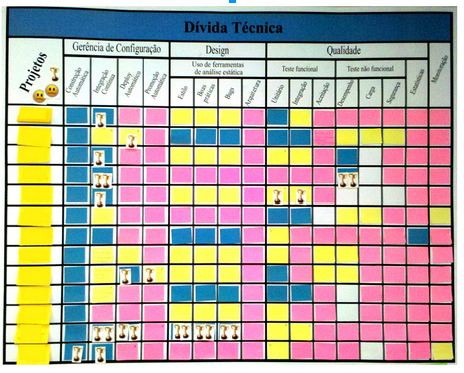
\includegraphics{images/DebtBoard}
	\centering
	\caption{Technical debt.}
	\label{fig:debtBoard}
\end{figure}


\subsection{Post-release quality}
\label{sec:PostQuality}
Metrics in post-release quality deal with evaluating the quality of the
product after it has been released.

Customer satisfaction, customer responsiveness, and quality indicators were
seen as attributes of post-release quality. Some metrics included customer
input to determine post-release quality
[S19,S7,S3] while other metrics
used pre-release data as predictors of post-release quality
[S25,S19,S7]. Customer related
metrics included, e.g., defects sent by customers [S3],
change requests from customers [S19] and customer's
willingness to recommend product to other potential customers
[S7].
Quality prediction metrics included defect counts [S19],
maintenance effort [S25] and deferred defect counts
[S7].

\subsection{Changes in processes or tools}
\label{sec:ChangesInProcesses}
This chapter describes the reported changes that applying metrics had for processes and tools. The changes include changes in measurement practices, development policies, and the whole development process.

The successful usage of sprint readiness metric and story flow metric changed
company policy to have target values for both metrics as well as monthly
reporting of both metrics by all projects [S13].

At Ericsson by monitoring the flow of requirements metric they decided to
change their implementation flow from push to pull to help them deliver in a
more continuous manner. Also, based on the metric they added an intermediate
release version to have release quality earlier in the development cycle.
[S20]

Changes to requirements management were also made based on lead time in other
case at Ericsson. Analysing lead time contributed to delaying technical design
after purchase order was received, providing customer a rough estimate quickly
and merging the step to create solution proposal and technical design.
[S18]

Problem with broken build, and the long times to fix the build, led to
measurements that monitor and visualize the state of the build and the time it
takes to fix it [S4,S13,S14].

Also, additional code style rules were added to code check-in and build tools
so that builds would fail more often and defects would get caught before
release [S13,S14]. 

Similarly, testing approaches were changed based on flow metrics. Using lead
time led to that integration testing could be started parallel to system
testing [S18]. Also, throughput of a test process showed
insufficient capability to handle the incoming features, which led to changing
the test approach [S26].

\begin{figure}
	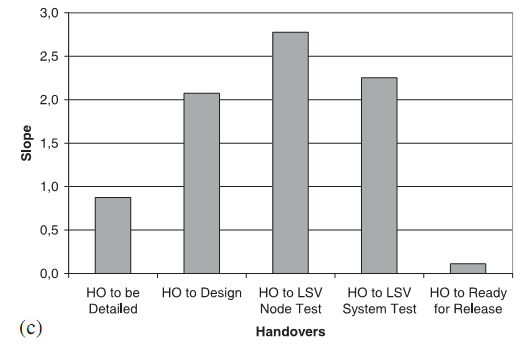
\includegraphics{images/HandoverPet2011}
	\centering
	\caption{Handovers [21]}
	\label{fig:handOvers}
\end{figure}

\end{comment}

\section{Metrics \& categorization}

Metrics are listed by primary study in appendix, see \Cref{tab:Metrics}.


Found metrics are categorized using categorization by
\citetsrc{fenton1998software}.

%    \begin{tabular}{p{2cm}p{7cm}p{5,5cm}} fenton kategorisoinnin taulukonkoko

% Table generated by Excel2LaTeX from sheet 'Taul1'
\begin{table}[htbp]
  \centering
  \caption{Add caption}
 	\begin{tabular}{p{2cm}p{7cm}p{5,5cm}}
    \toprule
    Entities & Attributes &  \\
    \midrule
    \textbf{Products} & \textbf{Internal} & \textbf{External} \\
    Product & Running tested features & Customer satisfaction x2, Net Promoter Score, numer of requests from customers, progress as working code \\
    Test plan & Number of test cases &  \\
    Code  & Technical debt in categories, technical debt in effort, violations of static code analysis &  \\
    Build & Build status x2, fix time of failed build &  \\
    Features & Remaining task effort, task's expected end date, task done, effort estimate x14, work in progress x3, number of days in maintenance, story complete percentage & Business value delivered, change requests per requirements \\
    Requirements & Implemented vs wasted requirements, requirement's cost types, Percentage of stories prepared for sprint &  \\
    Defects &       & Defect trend indicator, predicted number of defects \\
    \textbf{Processes} &       &  \\
    Testing & Defect count after testing, critical defects sent by customer, open defects x5, test success rate, test failure rate, faults per iteration, defects found in system test, defects deferred, test coverage, test growth ratio & Number of bounce backs, fault slips \\
    Implementation & Velocity x13, number of unit tests x4, completed web pages, cost performance index, schedule performance index, planned velocity, common compo time, average velocity & Story flow percentage \\
    Requirements engineering & velocity of elaborating features &  \\
    Whole development cycle & cycle time x2, lead time x4, processing time, queue time, maintenance effort, number of work items per phase x2, variance in handovers, rate of requirements per phase, throughput, queue, costs, schedule &  \\
    \textbf{Resources} &       &  \\
    Team  & Check-ins per day x3, actual effort & Team effectiveness \\
    Customer & Revenue per customer &  \\
    \bottomrule
    \end{tabular}%
  \label{tab:addlabel}%
\end{table}%

\fixme{Sano jotain j�rkev�� fentonin mukaan rakennetusta taulukosta.}

\begin{comment}
Metrics could help in decreasing software project failures due to
prioritization and resource \& schedule issues in iteration tracking. Metrics
here are all reactive.

Iteration tracking metrics could help in monitoring issues that lead to
project failures. Metrics are mostly reactive.

Metrics that are used to motivate and improve people can be used to solve
issues related to values \& responsibilities and company policies that lead to
project failures. Metrics are both reactive and proactive.

Metrics that are used to point identify problems can be used to prevent Method
causes for failures. Metrics are almost all proactive.

Metrics that are used to improve or understand pre-release quality can be used
to prevent failures that are caused by value \& responsibility, task output
and existing product related issues. Metrics are mostly reactive.

Metrics that are used for post-release quality can be used to prevent failures
that are caused by customers' and users' opinions. Metrics are mostly
proactive.

In general, used metrics were more reactive than proactive.

In general, it seems that metrics are used the most to prevent project
failures that are caused by Methods, then by Environment and not so much about
People or Tasks.
\end{comment}

\section{Why use metrics?}

Dokumentoi rajatapaukset why vs how, ja selit� niit�. esim balance of flow

\subsection{Identifying problems}

Metrics were used to identify bottlenecks in the process. Cumulative number of
work items over time metric was used to identify bottlenecks in the
development process [S22]. Monitoring Work-in-progress (WIP) was used to spot
blocked work items and also the development phase where the blockage occurred
[S2]. Cost types, rate of requirements over phases and variance in handovers
were for process improvement by spotting bottlenecks and uneven requirement
flows [S21].

Metrics were able to identify waste, development phases were no value is
added, in software processes. Value stream maps (VSM) were used to spot
waste in the development process [S18]. Lead time was used to identify waste
of waiting [S22]. Measuring story flow percentage allowed identification of
waste related to context shifts [S13].

Metrics were used to identify problems. Defect trend indicator was used to
provide the project manager an ISO/IEC 15939:2007 compatible indicator for problems with the defect backlog.
Basically, the indicator showed if the defect backlog will increase, stay the
same or decrease in the coming week [S25]. The project manager could then use
the info to take necessary actions to avoid possible problems. Schedule
performance index and cost performance index were used to monitor for deviances in the project's progress and providing early sign if something goes
wrong [S16]. Developers at Avaya had issues with the 80/20 rule, where the
last 20\% of iteration takes the longest [S29]. With the metrics that their
tool T3 provides (e.g Story percent complete) they were able to see the early symptoms
of various problems that can cause delays, and react early.

Metrics were also used to find improvement opportunities. Number of work items
per phase and lead time was used to spot instabilities in the process [S20].
If a measured value was outside the control limits it was defined an instability.
This enabled process improvement. Monitoring schedule and costs with a
dashboard allowed to spot for improvement opportunities at OCLC [S31].

\subsection{Planning}

Prioritization was one of the main activities metrics were used for. Effort
estimates were used to prioritize the features for next release and used as
basis for resourcing [S9]. Teams use effort estimates to prioritize activities
based on relative value and relative effort [S8]. At Verisign Managed Security
Services, they used many attributes to prioritize their backlog and revenue
per customer was described in more detail [S11]. At Timberline, they used Kano
analysis as a 'voice of customer' so that prioritization decision could be
based on facts instead of political power [S17]. Practitioners at Ericsson
used cost types, rate of requirements over phases and variance in handovers
for short term decisions related to requirements prioritization, staff
allocation and planning decisions [S21].

Metrics were used to estimate how many and how large features could be taken
under development. Velocity was used to improve effort estimates for next
planning session, and that way it was easier to understand how large can the
scope be for the next iteration [S16]. Leaders used estimates to check the if
the planned scope would be possible to complete during the next iteration
[S12]. At WMS, they used pseudo-velocity and average velocity to plan their
releases [S23]. Lead time was used to understand if all planned corrections
can be completed before release date [S24]. Story estimates were used to
understand the iteration where different features will be completed [S29].

Other planning uses for metrics were resourcing decisions and development
flexibility. At Timberline, they broke down requirements into smaller pieces
that were estimated in effort to understand what skills are needed to complete
the work [S17]. Marking tasks done and undone made it possible to take undone
tasks for the next iteration [S12]. Developers would mark expected end date
for task so the next one can plan their own work as effectively as possible
thus reducing idle time. Stories and their effort estimates were used as the
fundamental units of development for the iteration [S6]. Predicted number of
defects was used to plan the removal of defects. If the removal of defects
would not be well planned it could cause delays for the release and thus
increase costs for the project [S25].

\subsection{Progress tracking}

\subsubsection{Project progress}

Metrics were used to monitor the progress of the project. Completed web pages
was used as a measure of progress [S12]. Number of automated passing test
steps was used as a measure of progress in terms of completed work [S5].
Breaking down tasks to 'kits' between 2 to 5 days enabled progress monitoring
[S17]. Set of metrics(burndown, check-ins per day, number of automated passing
test steps, number of new and open defects) was developed to manage risks and
provide timely progress monitoring [S27]. Story percent complete metric was used to give assessment of
progress [S29]. A team at NASA Ames Reserch center didn't want to spend
resources on estimating features and instead focused on designing and
developing their software solution. Every six weeks they demonstrated their
progress to customer with working code [S30].

Other metrics were used to give higher level understanding of progress.
Release burndown shows project trends and can be used to predict completion
date [S16]. Release burndown also reflects addition or removal of stories.
Cost types, rate of requirements over phases and variance in handovers were
used to provide overview of progress [S21]. Metrics(burndown, check-ins per
day, number of automated passing test steps) were used to communicate
progress to upper management [S5] and ensure good progress to external
observers and ensure that key risks were under control [S5,S27,S28].

\subsubsection{Increase visibility}

Metrics were used to make complexity easier to understand and more visible.
Cost types, rate of requirements over phases and variance in handovers were
used to increase the transparency of end-to-end flow in a complex system
[S21]. Technical debt board was used to make technical debt issues visible and
easier to manage [S4]. Metrics(burndown, check-ins per
day, number of automated passing test steps, number of open and new defects)
were used to replace individual perception with facts [S27].

Metrics were used to keep the team informed. Defect trend indicator was used
to monitor defect backlog and spread the information to project members [S25].
Cycle time metrics were used to let the team track their own performance
[S23]. Story percent complete metric were generated automatically when tests
were run and thus kept everyone on the same page and eliminated schedule
surprises. The metric results were required to be reported periodically as
well [S29]. Release burndown made the correlation clear between work remaining
and team's progress in reducing it [S16].
 
\subsubsection{Accomplishing project goals}

Metrics were used to get understanding how the project is going in terms of
reaching goals. There was a need for simple indicator that would quickly tell
if project is under control. Common compo time was used to understand if
project was in target for delivery [S17]. Monitoring WIP was used predict lead
time which in turn will predict project schedule [S2]. Sprint burndown was
used to tell the team if they were on track regarding the sprint commitments
[S7]. Burndown was used to see if the team could meet their goals, and if not
what could be done [S5]. Story flow percentage was used so that developer
could finish a story in a steady flow [S13]. Burndown was used to mitigate the
risk where developers spend too much time perfecting features over finishing
all tasks of the iteration [S28].

\subsubsection{Balance workflow}

Metrics were used to balance workflow so that people working wouldn't feel
overloaded. Inventory of requirements over time was used to identify large
handovers of requirements that would cause overload situations. The aim was to
have steady flow of requirements [S20]. Operations department was overloaded
so they decided to start evaluating incoming work with Ops story points to
level the workload [S8]. People should be respected by having balanced
workload to avoid overload situations. Measuring number of requirements per
phase would help noticing peaks [S22]. Timberline tried to pace work according
to customer demand. However, too much work was pushed to development, which caused many problems, including
developers feeling overworked. They started using common tempo time to make
sure there would be balance of workflow [S17]. Component level burndown was
used to decide on resource mobility [S5].

Metrics were used solve large handovers. Variance in handovers was used to
guarantee that requirements would flow evenly [S21]. Mamdas was measuring
check-ins per day metric, which measured how often code is committed to main
trunk. The point was to avoid people from committing only at the end of the
iteration and instead integrate early and often [S5]. At WMS Gaming, they had
problems with large tasks blocking other work, so they set a rule that only
certain size of tasks(8 story points) can be taken for development [S23].

\subsection{Understand and improve quality}

\subsubsection{Understand level of quality}

Metrics were used to understand the level of quality after the release.
Net Promoter Score was measured because it was thought to be a pure measure of
success, since it's measured from the customers [S7]. Number of change
requests from customer was used as indicator customer satisfaction [S19].
Maintenance effort was used as an indicator of overall quality of the release
product [S19]. Number of maintenance requests was used as an indicator of
built in quality [S22].

Metrics were also used to understand the level of quality before the release.
Faults per iteration were used to measure the product's quality [S5]. Defects
found in system test was used to measure the quality of software delivered to
system test process [S7]. Defects deferred was used to predict the quality
customers would experience [S7].

\subsubsection{Increase quality}

Metrics were used to increase the level of quality. Governance mechanisms,
which included a set of metrics (burndown, check-ins per day and number of
automated passing test steps), were used to increase product quality [S28].
At T-Systems International, they used a set of metrics(build status, number of
unit tests, test coverage, test growth ratio, violations of static code
analysis) to improve project's internal software quality [S14]. Critical
defects sent by customers were tracked and fixed to prevent losing customers
[S3]. Build status was measured to prevent defects reaching production
environment [S14]. Violations of static code analysis was used to prevent the
existence of critical violations [S14]. Technical debt board was used to
reduce technical debt [S4].

\subsubsection{Ensure level of testing}

Metrics were used to make sure product is tested enough.
Test coverage was used to evaluate how well was the code tested [S14].
However, in Brown-field(legacy) projects it's better to measure
test-growth-ratio since there might be not be that many tests in the existing
code base. Work in progress was measured so it could be minimized. Otherwise
there would be problems e.g when there would be lot of untested code [S17].
Using number of automated passing test steps dealt with decreasing the risk
that the product would be un-thoroughly tested [S5]. Similarly, number of
automated passing test steps was used to make sure regression tests are ran
and passed every iteration [S5]. Story percent complete metric supports test
driven development [S29].

\section{What kind of effects did the use of metrics have?}

\subsection{Create improvement ideas}

This sections describes improvement ideas that were created based on metrics.

When a waste of extra process(requirement would wait for long time before full
specification) was identified in requirement specification with the help of
lead time, processing time and queue time metrics, a solution idea was created
where a quick high level proposal would be sent to customer without the need
for in-depth specification [S18]. Customer could then use the high level
proposal to evaluate if they want to pursue that requirement further. Similarly, two
requirement specification phases could be combined when another waste of extra
process was identified in requirements specification phase [S18].
Additionally, lead time could be decrease by increasing the collaboration with the market
unit and the development unit [S18]. Similarly, there was a waste of waiting
in design which could be improved by starting real work only when the
purchase order is received, not when requests are received [S18]. 

Lead time, processing time and queue time metric were used to identify waste
of waiting in testing phases [S18]. The improvement suggestion was to provide
earlier beta version and making testing phases parallel. Many of the
improvement ideas came from meetings where the value stream maps (VSM) were
used as a base for discussion.

Cost types, rate of requirements over phases and variance in handovers were
used to identify bottlenecks at Ericsson [S21]. They noticed that focusing on
deadlines caused a lot of requirements to be transferred to system test phase
close to the deadline. The improvement suggestion was to focus more on
continuous delivery instead of focusing on market driven deadlines.
Furthermore, Kanban was suggested as a development method to accomplish the
continuous delivery capabilities.

Throughput and queue time metrics were used to identify bottleneck in network
integration test phase which lead to using other testing practices in future
projects [S26].

Rate of requirements over time was used to identify problems in the
development process [S20]. One improvement suggestion was to change from push
to pull-approach so that team can adjust the workload to enable continuous
delivery. Another improvement suggestion was to add intermediate release
versions so that integration and testing would happen more often and problems
could be identified earlier than close to the actual release. Similar solution
was applied at Timberline inc. where requirements inventory was kept low which
meant that design, implementation and testing could start earlier and problems
in requirements would get caught sooner [S17].

Citrix online started measuring velocity for their Operations department
as well [S8]. This led to other departments trying to decrease their products'
Ops story points to enable faster releases. The reduction in story points was
possible by creating hot deployment strategies and providing better
documentation. 

Mamdas, an Israel Air force IT department, were using burndown to follow their
progress [28]. However, when they noticed that work remaining wasn't
decreasing according to remaining resources they had to make changes. In their iteration
summary meeting they decided to pursue senior engineers to help them create
optimal development environments and continuous build systems. Also, they
decided to evaluate customer requests in more detail to avoid over polishing
features. 

When story implementation flow metric showed a drop and project managers
complained about clarifications about features from customer were late, a root
cause analysis meeting was held [S13]. Also, after starting to use the
implementation flow metric new policies were stated to keep the flow
high: percentage of stories ready for sprint must be 100\% and implementation
flow must be at least 60\%, and both of the metrics need to be reported
montly. Root cause analysis was also conducted to decrease the amount of
bounce backs at Timberline inc. [S17].

A team noticed their velocity estimations were inaccurate which led to
dividing work items into smaller pieces to improve the accuracy of the
estimates [P10].

The reasons for the values of metrics(burndown, check-ins per day, number of
automated passing test steps, number of new and open defects) were discussed
in iteration summary meeting because it can be hard to analyze metrics without understanding the context
[S27]. Similarly, number of work items per phase was used to ask development
unit about the values of the metric and the development unit confirmed that
people felt overloaded as the metric suggested [S20]. Furthermore, if the
values of number of work items were outside the control limits one could
discuss with the developers about the workload [S22].

After analyzing long fix times for broken builds the team added
automatic static code analysis checks to code check-in to catch defects
earlier [S13]. Quality manager can change coding style guide and code
standards based on the results of violations to static code analysis metric
[S14].

\subsection{Planning actions}

Product owners use lead time to schedule high priority features and plan demo
dates with customers [S23]. Using revenue per customer metric allowed higher valued features to be
prioritized higher in the backlog. [S11] 

Velocity / 2 metric was used as scoping tool for a release. The team had
enough work not to sit idle, but there was still enough time to allow high
priority bug fixes to be fixed [S23]. Effort estimates are used to scope the
iteration and if there are tasks that cannot be completed before release date
then they are excluded from the backlog [S12]. Velocity was used to define
minimum delivery level for the iteration where 'must have' requirements are assigned, and a stretch goal where lower priority
requirements are assigned [S2].

Expected date of completion was used so that other team members could plan
their own work [S12].

\subsection{Reactive actions}

Metrics were used to cut down the scope or add more resources if it seemed not
all tasks could be completed with current pace. When component level burndown
was used to notice that a component was behind schedule, resources were added
and scope was reduced for the release [S5]. Release burndown showed that work remaining was not decreasing fast enough so
the scope of the release was decreased [S16]. If common compo time would show too much work, then tasks would be cut or more
resources would be added [S17]. Similarly, if work balance is uneven, some
roles have too much work while some don't have enough, people were trained in
multiple roles, e.g customer support did testing and documentation engineers
were taught how to input their material into the system. If team effectiveness
is not high enough to complete tasks, resources from other teams can be used. Other actions that were suggested were reduction of
tasks and working overtime [S3].


Metrics were also used to react to quality information. Monitoring cycle times
revealed high time consumption on manual testing [S17]. The cause was an
unmotivated person who was moved to writing automated test scripts which he
liked more. Number of defects were used to delay a release when too many
defects were noticed in a QA cycle [S10]. Quality manager interpreted results
of static code analysis from the build tool and he would then make plans for
necessary refactorings [S14]. When amount of written and passed unit tests was
not increasing an alarm was raised, when the issue was discussed in a
reflection meeting they understood that too much work was put to a single
tester writing the tests and once she was doing work for another project no
tests were written [S28]. The team then started to learn to do them on their
own as well, and later a dedicated tester was assigned to write the tests.


\subsection{Motivate people}

Metrics were used to motivate people to react faster to problems. Number of
defects was shown in monitors in hallways and that motivated developers to fix
defects [S3]. Total reported defects and test failure and success rate was
also shown throughout the organization which motivated people to avoid
problems and also fix problems fast [S3]. Fix time of failed build metric
improved people's mindset to react to problems immediately [S13]. The metric
was declared mandatory for all projects. Also, the reasons for long fix times
were investigated. Build status was visible in minutes after commits, which
helped to create a culture to react with high priority to broken builds [S4].
This helped to keep the main branch to be closer to deployable state at all
times. Build status was used to motivate people to fix the build as fast as
possible [S4]. Violations of static code analysis cause developers to
immediately fix the issue because the violations can cause a broken build
status [S14]. Additionally, developers get faster feedback on their work.
Furthermore, developers have more confidence in performing major refactorings
with the safety net the violations of static code analysis metric provides.


Metrics were used to change people's behavior. After meetings where technical
debt categories were analyzed, team members agreed which categories they would
focus in decreasing until the next meeting [S4]. Also, team members sought
help from the architecture team for reducing technical debt, e.g by
implementing automatic deployment or improving source code unit testability.
Measuring the number of automated passing test steps changed teams behaviour
to write more tests [S5]. Metrics were also used to prevent harmful behaviour
such as cherry picking features that are most interesting to the team [S17].
Measuring work in progress (WIP) and setting WIP limits prevented cherry
picking by enforcing only two features at a time and thus preventing them from
working on lower priority but more interesting features. Defect trend
indicator created crisis awareness and motivated the developers to take
actions in hopes to avoid possible problems [S25].

There can also be negative effects in using metrics. Using velocity metric had
negative effects such as cutting corners in implementing features to maintain
velocity with the cost of quality [S6].



\section{Important metrics in terms of statements}
 
This section describes metrics that were considered important.

Progress as working code was considered as one of the cornerstones of agile
[S30].

\begin{comment}
Capacity as number of features developed in release was considered better than
measuring speed, since speed is generally thought as a attribute of humans.
Capacity on the otherhand measures the capabilities of an organization.
\end{comment}

Story flow percentage and velocity of elaborating features were considered as
key metrics for monitoring projects. Also, a minimum 60\% value for flow was
identified. Similarly, velocity for elaborating features should be as fast as
velocity of implementing features. Also, they said using both metrics
\emph{``drive behaviors to let teams go twice as fast as they could before''}.
[S13]

Net Promoter Score was said to be \emph{``one of the purest measures of
success''} [S7].

According to a survey, projects that were said to be definitely successful
77\% measured customer satisfaction often or always. Also, the more often
customer satisfaction would be measured the more likely it would be that the
project would have good code quality and the project would succeed. [S1]

Story percent complete metric was considered valuable since it embraces test
driven development - no progress is made before test is written. Also, percent
complete metric is considered more accurate than previously used metric.
Moreover, it gives normalized measure of progress compared to developer
comments about progress. Additionally, story percent complete metric leverages
existing unit testing framework and thus requires only minimal overhead to
track progress. Team members seemed to be extremely happy about using the
metric. [S29]

Pseudo-velocity was considered essential for release planning [S23].

In an agile survey [S1], project success had significant positive
relationship with the following metrics: team velocity, business value
delivered, running testing features, defect count after testing and number of test cases.
However, there were no detailed descriptions of these metrics. 

Effort estimates were consider important in release planning especially in
terms of prioritization [S9].

Burndown was valuable in meeting sprint commitments [S7].
Similary, managers said burndown was important in making decisions and
managing multiple teams [S5]. However, developers didn't
consider burndown important [S5].

Top performing teams at Adobe estimated backlog items with relative effort
estimates [S7].

Practitioners at Ericsson valued transparency and overview of progress that
the metrics were able to provide to the complex product development with
parallel activities, namely cost types, rate of requirements over phases and
variance in handovers [S21].

At another case at Ericsson Value Stream Maps (VSM) were used to visualize
problem areas and possible improvements. Practitioners valued how the maps
were easy to understand. Metrics that were used to build VSM were lead time,
processing time and queue time. [S18]

Defects deferred was seen as a good predictor of post-release quality because
it correlated with issues found by the customers [S7].

Defect prediction metrics predicted number of defects in backlog and defect
trend indicator were seen important to decision making, and their use
continued after the pilot period. Key attributes of the metrics were
sufficient accuracy and ease of use. [S26]

Technical debt board that visualized the status of technical debt in
categories was considered important because it gave a high level understanding
of the problems and it was then used to plan actions to remove technical debt.
It was proven to be useful in their context. [S4]

The following metrics were consider very useful in agile context: number of
unit tests, test coverage, test-growth ratio and build status. The benefit
for the number of unit tests is not well described except that it provides
\emph{``first insights''}. Test coverage provides info on how well the code is
tested. Test-growth ratio is useful in projects where old codebase is used as
basis for new features. Fixing broken builds prevents defects reaching
customers. [S14]

\subsection{Important metrics based on amount of evidence}

Effort estimation metrics were used in many cases, so it could be perhaps said
they are important since they provide scoping and prioritization.


\chapter{Discussion}
\label{sec:Discussion}

\section{Implications for practice}
To provide implications to practice the findings are mapped to the principles
of agile software development \citetsrc{beck2001agile} categorized by Patel \&
al. \citetsrc{1579312}. For each paragraph the naming by Patel et al. is used
and references to the agile practices is provided by numbers.

Communication and Collaboration (principles 4 and 6) was reflected in metrics
that motivated a team to act and improve, see \cref{sec:Motivate}. Also,
progress metrics were used to communicate the status of the project to the
stakeholders, see \cref{sec:IterationTracking}.

Team involvement (5,8) was reflected in metrics that motivated team to act and
improve, see \cref{sec:Motivate}. Also, to promote sustainable development
metrics were targeted to balance the flow of work, see
\cref{sec:IterationTracking}.

Reflection (12) was visible in metrics that were used to identify problems and
to change processes, see \cref{sec:ProblemIdentification} and
\cref{sec:ChangesInProcesses}.

Frequent delivery of working software (1,3,7) was directly identified in one
paper, where the team measured progress by demonstrating the product to the
customer [S30]. Additionally, there were cases where e.g.
completed web-pages [S12] were the primary progress measure. Also, many
metrics focused on progress tracking and timely completion of the iteration, see \cref{sec:IterationTracking}. However, some other
measures from \cref{sec:IterationTracking} show that instead of working code
agile teams followed completed tasks and velocity metrics. 

%\juha{haluaisin jotain t�m�nkaltaista keskustelua suorista laatumittareista,
% mutta voiko n�in sanoa t�m�n tutkimuksen perusteella. Eetu, etenkin tuo
% viimeinen virke, onko linjassa sinun mielest�si??}\eetu{Nyt muokattuna voi
% sanoa.}
An integral part of the concept of working software is measuring post-release
quality, see  \cref{sec:PostQuality}. This was measured by customer
satisfaction, feedback, and customer defect reports. It was also common to use
pre-release data to predict post-release quality. Agile developers tend to
measure the end product quality with customer based metrics instead of the
traditional quality models, such as ISO/IEC 25010 \citepsrc{10951538}.

Managing Changing Requirements (2) was seen in the metrics that support
prioritization of features each iteration, see \cref{sec:IterationPlanning}.
Additionally, different metrics helped keeping the internal quality of the
product high throughout the development which then provided safe development
of modifications from new ideas, see \cref{sec:PreQuality}.

Design (9,10,11) was seen in focus to measuring technical debt and using
metrics to enforce writing tests before actual code, see
\cref{sec:PreQuality}. Additionally, the status of build was continuously
monitored, see \cref{sec:ChangesInProcesses}. However, the use of velocity
metric had a negative effect on technical quality, see
\cref{sec:IterationTracking}.
% was seen from different perspectives: on one hand metrics focused on
% problem/waste identification, see \cref{sec:ProblemIdentification},
Many metrics focused on making sure that the right features were selected for
implementation, see \cref{sec:IterationPlanning}, thus avoiding unnecessary
work.

\begin{comment}

Agile principle \#1: ``Our highest priority is to satisfy the customer through
early and continuous delivery of valuable software.'' was seen in the team
measuring progress by demonstrating the product to the customer
\cite{S30}.

Agile principle \#2: ``Welcome changing requirements, even late in
development. Agile processes harness change for the customer's competitive
advantage.'' was seen in the metrics that support prioritization of features
per iteration, see \cref{sec:IterationPlanning}. Additionally, different
metrics helped keeping the internal quality of the product high throughout the
development which then provided safe development of modifications and new
ideas, see \cref{sec:PreQuality}.

Agile principle \#3: ``Deliver working software frequently, from a couple of
weeks to a couple of months, with a preference to the shorter timescale''  was
seen in many metrics focusing on tracking and timely completion of the
iteration, see \cref{sec:IterationTracking}

Agile principle \#4:``Business people and developers must work 
together daily throughout the project.'' was seen how different metrics
were used to share information to all stakeholders about the project, see
\cref{sec:Motivate} and \cref{sec:IterationTracking}. 

Agile principle \#5:``Build projects around motivated individuals. Give them
the environment and support they need, and trust them to get the job done''
was reflected in metrics that motivated team to act and improve, see
\cref{sec:Motivate}.

Agile principle \#6:``The most efficient and effective method of 
conveying information to and within a development 
team is face-to-face conversation.'' was seen in \cite{S4} where
a technical debt board measuring the level of technical debt was used to
facilitate face-to-face discussion on technical debt issues, see
\ref{sec:PreQuality}. 

Agile principle \#7:``Working software is the primary measure of progress'' 
was directly identified in one paper, where the team measured progress by
demonstrating the product to the customer. Additionally, there were cases
where for example completed web-pages \cite{S12} were the primary
progress measure. However, some other measures from \cref{sec:IterationTracking} show that instead of working code agile teams followed completed tasks and velocity metrics.

Agile principle \#8:``Agile processes promote sustainable development. The
sponsors, developers, and users should be able to maintain a
constant pace indefinitely.'' was followed with metrics targeted to balance
the flow of work, see \cref{sec:IterationTracking}.

Agile principle \#9:``Continuous attention to technical excellence 
and good design enhances agility.'' was seen in focus to measuring technical
debt and using metrics to enforce writing tests before actual code, see
\cref{sec:PreQuality}. Additionally, the status of build was continuously
monitored, see \cref{sec:ChangesInProcesses}. However, the use of velocity
metric had a negative effect on technical quality, see
\cref{sec:IterationTracking}.

Agile principle \#10:``Simplicity---the art of maximizing the amount 
of work not done---is essential.'' was seen from different perspectives: on one
hand metrics focused on problem/waste identification, see
\cref{sec:ProblemIdentification}, and on the other hand many metrics focused
on making sure that the right features were selected for implementation, see
\cref{sec:IterationPlanning}.

Agile principle \#11:``The best architectures, requirements, and designs
emerge from self-organizing teams.'' was seen in metrics that motivate the
team to improve, see \cref{sec:Motivate}. Other perspective is that since
effort estimation is done by the team, the team is then more motivated to
accomplish the goal, see \cref{sec:IterationPlanning}.

Agile principle \#12: ``At regular intervals, the team reflects on how to
become more effective, then tunes and adjusts its behavior accordingly'' was
visible in metrics that were used to identify problems and to change
processes, see \cref{sec:ProblemIdentification} and 
\cref{sec:ChangesInProcesses}.

\end{comment}

%\eetu{Mun mielest� seuraavat mittarit ei oo niin ketteri�, mut en osaa oikeen
%perustella miksi tai sanoa mit� periaatteita vastaan ne olisi: maintenance
%effort, cost types, defect amounts(?), defects deferred, revenue per
%customer(?), time to establish project foundation, test coverage, test growth
%ratio, cost performance index, schedule performance index. N�it� ei kaikkia
%ole my�sk��n kuvattu resultseissa, paitsi taulukossa mainittu.}

There were also metrics, or their usage, which were not agile in nature. E.g.,
maintaining velocity by cutting corners in quality instead of dropping
features from that iteration [S6]. Also, adding people to
project to reach a certain date [S5, S17] doesn't seem that
agile compared to removing tasks. Adding people can have a negative impact to
progress, considering the lack of knowledge and training time required.
Moreover, the use of dates to plan interdependent tasks is not agile in
nature [S12]. Instead, interdependencies should be visible in
choosing the tasks to appropriate iterations. Also, the use of number of
defects to delay a release [S10] is against agile thinking
as one should rather decrease the scope to avoid such a situation.

%While the flow metrics Ericsson have a good target of balancing workflow,
% they seem  (or at least they are presented) complicated to use---meaning that one
%might need considerable effort to generate and analyse the metrics, which
%doesn't fit to the light-weightness of agile.

%\juha{muotoilisin t�m�n hieman toisin}
% Contradictory to fifth principle, Talby et al [viite] enforce writing
% automated test cases as a measure of progress - so in a way they didn't
% trust the developers to write the test on their own? Similarly, [viite]
% measured the status of the build to make developers fix the build faster -
% again, not trusting them to do it on their own.
Some agile metrics that work well for an agile team, such as tracking progress
by automated tests [S28], or measuring the status of the build
[S14] can turn against the agile principles if used as an external
controlling mechanism. The fifth agile principle requires trust in the team,
but if the metrics are enforced outside of the team, e.g., from upper
management there is a risk that the metrics turn into control mechanisms and
the benefits for the team itself suffer.

%\subsection{Implications for research}
%It was interesting to notice that there wasn't many code metrics, only the
%ones mentioned in \cite{S14} even though we feel there are many
%% studies regarding the benefits of code metrics. Maybe there are some
% practical
%problems implementing and analysing the data from code metrics?

%How to measure unmeasured agile principles...

%Effort estimates are prerequisite for velocity metrics, and since velocity
%metrics were vastly identified in our study, e

%In general, we think there were many metrics that were targeted for the team
% - instead of high focus on managerial or upper management reporting metrics.
%Making metrics visible for the team enables them to independently act and
%improve without the need of rapid supervision and telling people what to do.

\subsection{Comparison to prior studies}
Only few papers have broadly studied the reasons for software metrics use in
the context of agile software development. \citetsrc{1667571} also highlight process improvement as one of the reasons
for measurement in their agile metrics paper. Also, they emphasize that creation of value should
be the primary measure of progress - which was also seen in this study.

\citetsrc{Korhonen2009} found in her study that traditional defect
metrics could be reused in agile context - if modified. Defect metrics were
also used in many of the primary studies.

Kitchenham's mapping study \citepsrc{kitchenham_whats_2010} identified several
code metrics in academic literature. However, in this study almost no evidence
of code metric use in the industrial agile context was found. Maybe agile
practitioners consider code metrics self-evident and don't report them, or
maybe code metrics aren't widely used by agile industrial teams.

%Maybe it is time to
%re-evaluate the need for code metrics research if industry doesn't seem to
% use them.

%The reasons for the lack of code metric usage in agile
%contexts should be studied to evaluate the necessity of code metric research
% - or how code metric research could be modified to support agile development

%The lone case in our study where code metrics were used, the code
%metric usage was abstracted to a build tool, which would just indicate an
%error or broken build \cite{S14}. Maybe the use of code metrics should
%be heavily implemented through automated tools that handle the collection and
%analysing of code metric data?


\section{Limitations}

\fixme{Add SLR vs survey - eli p�hk� tutkimusmenetelm� valittu teht�v��n}
The large shares of specific application domains in the primary documents is a
threat to external validity. Seven out of 29 studies were from enterprise
information systems domain and especially strong was also the share of ten
telecom industry studies out of which eight were from the same company,
Ericsson. Also, Israeli Air Force was the case organization in three studies.

The threats to reliability in this research include mainly issues related to
the reliability of primary study selection and data extraction. The main
threat to reliability was having a single researcher performing the study
selection and data extraction. It is possible that researcher bias could have
had an effect on the results. This threat was mitigated by analysing the
reliability of both study selection and data extraction as described in
\cref{sec:Method}.

%Sometimes it was hard to understand which metrics an author was referring
%when a ``why'' was described. Moreover, we had to sometimes assume that when
%author describes the reasons for using a tool, he would be actually talking
%about the metrics the tool shows.

Due to iterative nature of the coding process, it was challenging to make sure
that all previously coded primary documents would get the same treatment,
whenever new codes were discovered. In addition, the researcher's coding
``sense'' developed over time, so it is possible that data extraction accuracy
improved during the analysis. In order to mitigate these risks a pilot study
was conducted to improve the coding scheme, get familiar with the research
method, refine the method and tools.

%First author has positive mindset towards agile methods, as well as towards
%certain metrics over others.

Some data from low scoring papers, e.g [S3], are not justified very
detailed which could cause incorrect interpretations.


\chapter{Conclusions}%\juha{Kirjoitin t�nne hieman lis��...} 
\label{sec:Conclusions}

This study presents the results from a systematic literature review from 29
\fixme{numero}primary studies. According to the researcher's knowledge there
is no previous systematic reviews of measurement use in the context of
industrial agile software development. This study classifies and describes the
main measurement types and areas that are reported in empirical studies. This
study provides descriptions of how and why metrics are used to support agile
software development.\fixme{lis�� important metrics ja metrics categories}
This study also analyzed how the presented metrics support the twelve
principles of Agile Manifesto \citepsrc{beck2001agile}.

The results indicate that the reasons and use of metrics is focused on the
following areas:
\nameref{sec:IterationPlanning}, \nameref{sec:IterationTracking},
\nameref{sec:Motivate}, \nameref{sec:ProblemIdentification},
\nameref{sec:PreQuality}, \nameref{sec:PostQuality} and
\nameref{sec:ChangesInProcesses}.

This paper provides researchers and practitioners with an useful overview of
the measurements use in agile context and documented reasonings behind the
proposed metrics. This study can be used as a source of relevant sources
regarding researchers' interests and contexts.

Finally, this study identified few propositions for future research on
measuring in agile software development. First, in the academia lot of
emphasis has been given to code metrics yet this study found little evidence
of their use in agile context. Second, the applicable quality metrics for
agile development and the relationship of pre-release quality metrics and post-release quality are
important directions of future research. Third, this study found that planning
and tracking metrics for iteration were often used indicating a need to focus
future research efforts on these areas. Fourth, use of metrics for motivating
and enforcing process improvements can be an interesting future research
topic.

\fixme{Add future work - negative effects of metrics. negative motivation
effects of metrics.}

\fixme{lis�� important metrics ja metric categories}





% Load the bibliographic references
% ------------------------------------------------------------------
% You can use several .bib files:
%\bibliography{sources}
%\bibliographystylesrc{plain}

%\addcontentsline{toc}{chapter}{\refname}  % article

\bibliographysrc{sources}


\chapter*{Primary studies}
\addcontentsline{toc}{chapter}{Primary studies}  



\begin{supertabular}{ l p{14.2cm} }
    {[}S1{]} & N\bibentry{S1} \\ [2ex] \shrinkheight{-6cm}
    {[}S2{]} & D\bibentry{S2} \\ [2ex]
    {[}S3{]} & T\bibentry{S3} \\ [2ex]
    {[}S4{]} & P\bibentry{S4} \\ [2ex]
    {[}S5{]} & Y\bibentry{S5} \\ [2ex]
    {[}S6{]} & A\bibentry{S6} \\ [2ex]
    {[}S7{]} & P\bibentry{S7} \\ [2ex]
    {[}S8{]} & D\bibentry{S8} \\ [2ex]
    {[}S9{]} & N\bibentry{S9} \\ [2ex]
    {[}S10{]} & P\bibentry{S10} \\ [2ex]
    {[}S11{]} & P\bibentry{S11} \\ [2ex]
    {[}S12{]} & N\bibentry{S12} \\ [2ex] \shrinkheight{-5cm}
    {[}S13{]} & C\bibentry{S13} \\ [2ex]
    {[}S14{]} & A\bibentry{S14} \\ [2ex]
    {[}S15{]} & V\bibentry{S15} \\ [2ex]
    {[}S16{]} & P\bibentry{S16} \\ [2ex]
    {[}S17{]} & S\bibentry{S17} \\ [2ex]
    {[}S18{]} & K\bibentry{S18} \\ [2ex]
    {[}S19{]} & K\bibentry{S19} \\ [2ex]
    {[}S20{]} & K\bibentry{S20} \\ [2ex]
    {[}S21{]} & K\bibentry{S21} \\ [2ex]
    {[}S22{]} & R\bibentry{S22} \\ [2ex]
    {[}S23{]} & M\bibentry{S23} \\ [2ex]
    {[}S24{]} & M\bibentry{S24} \\ [2ex]
    {[}S25{]} & M\bibentry{S25} \\ [2ex]
    {[}S26{]} & M\bibentry{S26} \\ [2ex]
    {[}S27{]} & D\bibentry{S27} \\ [2ex]
    {[}S28{]} & D\bibentry{S28} \\ [2ex]
    {[}S29{]} & V\bibentry{S29} \\ [2ex]
    {[}S30{]} & J\bibentry{S30} \\ [2ex] 
    {[}S31{]} & D\bibentry{S31} \\
\end{supertabular}

%\bibliographysec{lahteet_s}




% Appendices go here
% ------------------------------------------------------------------
% If you do not have appendices, comment out the following lines
\appendix
\chapter{Search strings}
\label{app:Strings}

The first search string was:

TITLE-ABS-KEY(software AND (agile OR lean OR "crystal method" OR "crystal
clear" OR dsdm OR "dynamic systems development method" OR fdd OR "feature
driven development" OR "agile unified process" OR "agile modeling" OR scrumban
OR kanban OR scrum OR "extreme programming" OR xp) AND (measur* OR metric OR
diagnostic OR monitor*)) AND (LIMIT-TO(SUBJAREA, "COMP")) AND
(LIMIT-TO(LANGUAGE, "English"))\\

It found 512 hits 19 September 2013.\\\\

%Then we noticed that some previously found key papers were missing from the
%hits because they were under sub area ``Engineering'', thus 
The second search string was:\\

TITLE-ABS-KEY(software AND (agile OR lean OR "crystal method" OR "crystal
clear" OR dsdm OR "dynamic systems development method" OR fdd OR "feature
driven development" OR "agile unified process" OR "agile modeling" OR scrumban
OR kanban OR scrum OR "extreme programming" OR xp) AND (measur* OR metric OR
diagnosticOR monitor*)) AND (LIMIT-TO(LANGUAGE, "English")) AND
(LIMIT-TO(SUBJAREA, "ENGI")) AND (EXCLUDE (SUBJAREA, "COMP") OR
EXCLUDE(SUBJAREA, "PHYS") OR EXCLUDE(SUBJAREA,"MATE") OR EXCLUDE (SUBJAREA,
"BUSI") OR EXCLUDE(SUBJAREA, "MATH") OR EXCLUDE(SUBJAREA, "ENVI") OR
EXCLUDE (SUBJAREA, "EART") OR EXCLUDE(SUBJAREA, "DECI") OREXCLUDE (SUBJAREA,
"ENER"))\\

It found 220 hits 7 November 2013.\\\\

The third search string was:\\

TITLE-ABS-KEY(software AND (agile OR lean OR "crystal method" OR "crystal
clear" OR dsdm OR "dynamic systems development method" OR fdd OR "feature
driven development" OR "agile unified process" OR "agile modeling" OR scrumban
OR kanban OR scrum OR "extreme programming" OR xp) AND (measur* OR metric OR
diagnosticOR monitor*)) AND (LIMIT-TO(LANGUAGE, "English")) AND
(LIMIT-TO(SUBJAREA, "BUSI")) AND (EXCLUDE (SUBJAREA, "ENGI") OR
EXCLUDE(SUBJAREA, "COMP"))\\

It found 42 hits 10 December 2013.

\chapter{Inclusion and exclusion criteria}
\label{app:Criteria}

Inclusion criteria
\begin{itemize}
  \item Papers that present the use and experiences of metrics in an agile
  industry setting.
\end{itemize}

Exclusion criteria
\begin{itemize}
  \item Papers that do not contain empirical data from industry cases.
  \item Papers that are not in English.
  \item Papers that do not have agile context. There is evidence of
  clearly non-agile practices or there is no agile method named. For example,
  paper mentions agile but case company has only three releases per year.
  \item Paper is only about one agile practice, which is not related to
  measuring.
  \item Papers that do not seem to have any data about metric usage.
  Similarly, if there are only a few descriptions of metrics but no other info regarding
  reasons or usage.
  \item Papers that have serious issues with grammar or vocabulary and
  therefore it takes considerable effort to understand sentences.
  %\item Papers that refer to another paper where the actual case is discussed.
  %\item Papers that are in academic or semi-academic setting - customer or
  %part of workers are from industry. The reason for this is that it doesn't
  %fully represent industry setting as software development methods are likely
  %enforced by academia. \juha{t�m� sis�ltyy tai vain tarkentaa ensimm�ist�}
  \item Papers where the setting is not clear or results cannot be separated by setting, for example
  surveys where there is data both from academia and industry. %Similar
%  exclusion if results cannot be separated by software development method. 
  %\item Papers where the setting is not clear. For example only mention of
  %context is ``100 junior developers''.\juha{yhdistin edelliseen}

  %%\item Papers that are full conference proceedings. Individual papers should be already listed separately.
  \item Papers where the metrics are only used for the research. For
  example, author measures which agile practices correlate with success.
  %%\item Papers that don't even show measurement usage in a pilot setting. For
  %%example method or metric is used against static industrial data set. \juha{t�m� sis�ltyy tai vain tarkentaa ensimm�ist�}
\end{itemize}

\chapter{Quality assesment questions}
\label{app:quality}

Based on the quality evaluation form by \citetsrc{dyba_empirical_2008}.

\begin{enumerate}
  \item Is this a research paper?
  \item Is there are a clear statement of the aims of the research?
  \item Is there an adequate description of the context in which the research
  was carried out?
  \item Was the research design appropriate to address the aims of the
  research?
  \item Was the recruitment strategy appropriate to the aims of the research?
  \item Was there a control group with which to compare treatments?
  \item Was the data collected in a way that addressed the research issue?
  \item Was the data analysis sufficiently rigorous?
  \item Has the relationship between researcher and participants been
  considered adequately?
  \item Is there a clear statement of findings?
  \item Is the study of value for research or practice?
\end{enumerate}

\chapter{Definions of metrics}
\label{app:definitionsOfMetrics}

% Table generated by Excel2LaTeX from sheet 'DefinitionsOfMetrics'

{\small
\begin{longtable}{p{1,5cm}p{3cm}p{7,5cm}} 
\caption{Definitions of found metrics}\\
\toprule\\
Primary study &     Metric & Definition \\
\midrule\\

     [S10] & \# of defects & Issues found from quality assurance cycle including variance from expected behavior. \\

      [S7] & \# of defects found in system test & Number of defects found in system test. \\

     [S25] & \# of defects in backlog & All known and unresolved defects in the project. \\

      [S7] & \# of open defects & Number of open defects on the current release per day. \\

     [S22] & \# of requirements per phase & Number of requirements per phase. \\

     [S14] & \# of unit tests & Number of unit tests. \\

     [S23] & Average velocity & Not clearly defined in primary study.  \\

 [S4, S14] & Build status & Build broken or not. \\

[S5, S27, S28] &   Burndown & Remaining human resource days versus the remaining work days. \\

      [S7] &   Burndown & Not defined in primary study.  \\

      [S1] & Business value delivered & Not defined in primary study. Probably means delivered features per timeframe. \\

     [S19] & Change requests per requirement & Amount of change requests from customer per requirement. \\

[S5, S27, S28] & Check-ins per day & Number of commits (code, automated test, specification) per day. \\

     [S17] & Common tempo time & Net working days available per number of units required. \\

     [S12] & Completed web pages & Completed web pages. \\

     [S16] & Cost performance index & Not defined in primary study.  \\

      [S3] & Critical defects sent by customer & Not defined in primary study.  \\

      [S1] & Customer satisfaction & Not defined in primary study.  \\

     [S17] & Customer satisfaction (Kano analysis) & Not clearly defined in primary study.  \\

     [S17] & Cycle time & Not defined in primary study.  \\

     [S23] & Cycle time & Time it takes for x size story to be completed. \\

      [S1] & Defect count after testing & Not defined in primary study. Probably means amount of defects after first round of testing. \\

     [S25] & Defect trend indicator & Indicates if amount of defects in the coming week will increase, stay the same or decrease from this week. \\

      [S7] & Defects deferred & Not defined in primary study. Probably means the amount of defects that are known but are not fixed for the release. \\

      [S9] & Effort estimate & Estimated effort per story in ideal pair days. \\

     [S12] & Effort estimate & Not clearly defined in primary study.  \\

[S15, S15, S15, S15] & Effort estimate & Not defined in primary study.  \\

     [S17] & Effort estimate kits & Tasks are broken down into kits of two to five staff-days of work. \\

     [S19] & Fault slips & Amount of issues that should have been found already in the previous phase. \\

      [S5] & Faults per iteration & Faults per iteration. \\

     [S13] & Fix time of failed build & Fix time of failed build. \\

     [S19] & Implemented vs wasted requirements & Ratio of implemented requirements and wasted requirements. Not all requirements are implemented but some work is put into them. \\

     [S20] & Inventory of requirements over time & Amount of requirements in specific work space over time. \\

     [S18] &  Lead time & The average time it takes for one request to go through the entire process from start to finish. \\

[S19, S22] &  Lead time & Time it takes for requirement to go through a sub-process or the whole process. \\

     [S24] &  Lead time & Not clearly defined in primary study.  \\

     [S19] & Maintenance effort & Costs related to fixing issues that have been found and reported by customers. \\

      [S7] & Net Promoter Score & Not defined in primary study. Probably measures how likely customers will recommend the product to another customer. \\

[S5, S27, S28] & Number of automated passing test steps & Number of automated passing test steps. \\

     [S17] & Number of bounce backs & Not defined in primary study. Probably the amount of defects that should have not occurred anymore if a root cause would have been fixed earlier. \\

     [S27] & Number of new and open defects & Number of new and open defects. \\

     [S20] & Number of requests from customers & Not defined in primary study.  \\

      [S1] & Number of test cases & Not defined in primary study.  \\

      [S3] & Open defects & Not defined in primary study.  \\

      [S8] & Operations' velocity & Not defined in primary study. Probably Operations department's completed story points per time unit. \\

     [S13] & Percentage of stories prepared for sprint & Percentage of stories prepared for sprint. \\

     [S16] & Planned velocity & Not clearly defined in primary study.  \\

     [S25] & predicted \# of defects & Predicted number of defects in backlog in the coming week. \\

     [S18] & Processing time & The time the request is being worked on by one person or a team. \\

     [S30] & Progress as working code & Product is demonstrated to the customer who then gives feedback. \\

     [S23] & Pseudo velocity & Not clearly defined in primary study.  \\

     [S26] &      Queue & Number of units remaining to be developed/processed by a given phase or activity. \\

     [S18] & Queue time & The average time between sub-processes that the request sits around waiting. \\

     [S21] & Rate of requirements per phase & Rate of requirements flow from a phase to next phase. \\

     [S16] & Release burndown & Amount of work remaining till the release. \\

      [S3] & Remaining task effort & Not defined in primary study.  \\

     [S21] & Requirement's cost types & Cost distribution of a requirement. \\

     [S11] & Revenue per customer & Amount of revenue from customer per feature.  \\

      [S1] & Running tested features & Not defined in primary study. Probably means amount of features delivered to customer that are passing unit tests. \\

     [S16] & Schedule performance index & Not defined in primary study.  \\

     [S16] & Sprint burndown & Amount of work remaining till the end of sprint. \\

     [S29] & Story complete percentage & Not clearly defined in primary study.  \\

     [S29] & Story estimate & Estimated days to complete the story. \\

      [S6] & Story estimates & Estimated time to develop a story. \\

     [S13] & Story flow percentage & Estimated implemention time per actual implemention time * 100. \\

      [S7] & Story points & Not defined in primary study.  \\

      [S8] & Story points & Estimated effort to complete the story in programmer days. \\

     [S12] &  Task done & Task done. \\

      [S8] & Task effort & Estimated effort to complete the task in programmer hours. \\

     [S12] & Task's expected end date & Date when a task is estimated to be finished. \\

      [S3] & Team effectiveness & Not defined in primary study.  \\

      [S4] & Technical debt board & Shows the status of each technical debt category per team. \\

      [S4] & Technical debt in effort & Technical debt in amount of hours it would take to fix all the issues increasing technical debt calculated by third party tool called Sonar. \\

     [S14] & Test coverage & How much Source Code executed during Test Execution. \\

      [S3] & Test failure rate & Not defined in primary study.  \\

     [S14] & Test growth ratio & Difference of amount of tests per difference of amount of Source Code. \\

      [S3] & Test success rate & Not defined in primary study.  \\

     [S26] & Throughput & Number of units processed by a given phase or activity per time. \\

     [S21] & Variance in handovers & Changes in amount of handed over requirements. \\

      [S2] &   Velocity & Amount of developed scenarios per developer per week. \\

      [S6] &   Velocity & Not defined in primary study.  \\

      [S8] &   Velocity & Not defined in primary study.  \\

     [S10] &   Velocity & Feature points developed per iteration. \\

     [S13] & Velocity of elaborating features & Not clearly defined in primary study. Probably the time it takes to clarify a feature from customer into requirements that can be implemented. \\

     [S13] & Velocity of implementing features & Not clearly defined in primary study. Probably the time it takes to implement a feature. \\

     [S14] & Violations of static code analysis & Amount of violations to static code analysis rules from tools like Findbugs, PMD and Checkstyle. \\

     [S17] & Work in progress & Amount of features or feature level integrations team is working on. \\

     [S23] & Work in progress & Amount of stories per work phase. \\

     [S24] & Work in progress & Amount of work items per phase. \\
     
     \bottomrule\\
     \label{tab:definitionsOfMetrics}

\end{longtable}  
}



% End of document!
% ------------------------------------------------------------------
% The LastPage package automatically places a label on the last page.
% That works better than placing a label here manually, because the
% label might not go to the actual last page, if LaTeX needs to place
% floats (that is, figures, tables, and such) to the end of the 
% document.
\end{document}
